\documentclass[]{politex}
% REMOVER LINHA ABAIXO PARA VOLTAR À FONTE NORMAL DO LATEX
\renewcommand{\familydefault}{\sfdefault}
% ========== Opções ==========
% pnumromarab - Numeração de páginas usando algarismos romanos na parte pré-textual e arábicos na parte textual
% abnttoc - Forçar paginação no sumário conforme ABNT (inclui "p." na frente das páginas)
% normalnum - Numeração contínua de figuras e tabelas 
%	(caso contrário, a numeração é reiniciada a cada capítulo)
% draftprint - Ajusta as margens para impressão de rascunhos
%	(reduz a margem interna)
% twosideprint - Ajusta as margens para impressão frente e verso
% capsec - Forçar letras maiúsculas no título das seções
% espacosimples - Documento usando espaçamento simples
% espacoduplo - Documento usando espaçamento duplo
%	(o padrão é usar espaçamento 1.5)
% times - Tenta usar a fonte Times New Roman para o corpo do texto
% noindentfirst - Não indenta o primeiro parágrafo dos capítulos/seções


% ========== Packages ==========
\usepackage[utf8]{inputenc}
\usepackage{amsmath,amsthm,amsfonts,amssymb}
\usepackage{graphicx,cite,enumerate}
\usepackage{blkarray}
\usepackage{float}
\graphicspath{ {imagens/} }

% ========== Language options ==========
\usepackage[brazil]{babel}
%\usepackage[english]{babel}


% ========== ABNT (requer ABNTeX 2) ==========
%	http://www.ctan.org/tex-archive/macros/latex/contrib/abntex2
\usepackage[alf]{abntex2cite}

% Forçar o abntex2 a usar [ ] nas referências ao invés de ( )
%\citebrackets{[}{]}




% ========== Opções do documento ==========
% Título
\titulo{net.map - Sistema de Posicionamento Indoor}

% Autor
%\autor{Nome Sobrenome}

% Para múltiplos autores (TCC)
\autor{Adriano Dennanni\\
Ricardo Nagano\\
Thiago Lira}

% Orientador / Coorientador
\orientador{Prof. Dr. Reginaldo Arakaki}
\coorientador{Eng. Marcelo Pita}


% Tipo de documento
\tcc{Eletricista com ênfase em Computação}

% Departamento e área de concentração
\departamento{PCS}
\areaConcentracao{Engenharia de Computação}

% Local
\local{São Paulo}

% Ano
\data{2016}




\begin{document}
% ========== Capa e folhas de rosto ==========
\capa
\falsafolhaderosto
\folhaderosto


% ========== Folha de assinaturas (opcional) ==========
%\begin{folhadeaprovacao}
%	\assinatura{Prof.\ X}
%	\assinatura{Prof.\ Y}
%	\assinatura{Prof.\ Z}
%\end{folhadeaprovacao}


% ========== Ficha catalográfica ==========
% Fazer solicitação no site:
%	http://www.poli.usp.br/en/bibliotecas/servicos/catalogacao-na-publicacao.html


% ========== Dedicatória (opcional) ==========
%\dedicatoria{Dedicatória}


% ========== Agradecimentos ==========
\begin{agradecimentos}

\end{agradecimentos}


% ========== Epígrafe (opcional) ==========
\epigrafe{

	\emph{``Anything one man can imagine, other men can make real''}
	\begin{flushright}
		-{}- Jules Verne
	\end{flushright}
	
	\hfill \break
	
	\emph{``Enquanto sentir vontade de competir, buscar desafios e correr atrás de torneios, vou jogar''}
	\begin{flushright}
		-{}- Gustavo Kuerten
	\end{flushright}
	
	\hfill \break
	
	\emph{``Not all those who wander are lost''}
	\begin{flushright}
		-{}- J. R. R. Tolkien
	\end{flushright}
}


% ========== Resumo ==========
\begin{resumo}

Mapas físicos tornam-se cada vez menos utilizados com o desenvolvimento progressivo
de sistemas de posicionamento cada vez melhores. O sistema americano
GPS é possivelmente o mais utilizado, sendo que ele possibilita qualquer um ter informações
sobre sua localização, dando apoio, por exemplo, à praticantes de trilhas e
acampamentos, principalmente em casos de emergência. Porém, em ambientes fechados,
as ondas eletromagnéticas utilizadas pelos satélites sofrem atenuações e interferências
devidos aos materiais de construção, e assim o sistema perde precisão e não
funciona com toda a precisão esperada. Como uma alternativa para esta dificuldade,
procurou-se desenvolver um sistema, que consegue obter a posição do usuário em um
ambiente fechado com precisão, sendo usado para isso técnicas de machine learning,
aliadas com dados obtidos de redes em fio já instaladas no local. O sistema consistirá
de um servidor central, onde serão enviados os dados e os mesmos serão processados.
Os dados serão coletados por meio de um aplicativo de Android, este possuirá
duas versões: versão de usuário final, que usará os dados do servidor para localizá-lo, e a
versão de administrador, que irá coletar dados novos para serem usados em futuras medições.
%
\\[3\baselineskip]
%
\textbf{Palavras-Chave} -- Localização Indoor, Wi-Fi, Machine Learning.
\end{resumo}

% ========== Abstract ==========
\begin{abstract}

Physical maps are becoming each day less used due to constant evolution of positioning
systems, better each day as well. The American system GPS probably is the
most used and the most famous. It allows everyone to have their location information,
giving support to hikers and campers, specially in emergency situations. On the other
hand, in indoor environments, electromagnetic waves used by the satellites suffer with
interference and mitigations and the systems loses precision and does not work as expected.
As an alternative for this difficulty, it was developed a system that can locate
the user position in an indoor environment with precision, using machine learning algorithms
and data of wireless signals collected from the networks already existing on
the place. The system consists on a main server that will receive the data and process
it. The data will be collected with a Android app that will have two versions. The user
version will use the server data to locate the user. The admin version will collect new
data to be user on future measures.
%
\\[3\baselineskip]
%
\textbf{Palavras-Chave} -- Indoor Location, Wi-Fi, Machine Learning.
\end{abstract}

% ========== Listas (opcional) ==========
\listadefiguras
\listadetabelas

% ========== Listas definidas pelo usuário (opcional) ==========
%\begin{pretextualsection}{Lista de símbolos}
%\end{pretextualsection}

% ========== Sumário ==========
\sumario


% ========== Elementos textuais ==========

\chapter{Introdução}\label{chp:introduction}

\section{Motivação}\label{sec:motivation}
Com a modernização das tecnologias de telefonia móvel torna-se cada vez maior o
número de pessoas com acesso à \textit{Internet}, através de tecnologias como \textit{Wi-fi},
3G e 4G. Essas formas de acesso à rede fornecem informações a provedores sobre o
usuário a todo momento,como o conteúdo acessado por seus navegadores ou aplicativos
e informações sobre posição e deslocamento. Dados de localização por si possuem
pouco valor, mas quando aliados a outros conteúdos, é possível fornecer conteúdo
personalizado em tempo real, reativo ao ambiente, passando a oferecer valor real
à empresas e entidades.
\par
Sistemas de posicionamento por satélite como GPS conseguem localizar um dispositivo
na Terra com uma precisão na casa dos centímetros em ambientes abertos. Porém,
o mesmo não ocorre em lugares fechados, como residências e edifícios. Isso ocorre
devido à atenuação dos sinais dos satélites causada pelas paredes e tetos das
estruturas. Tendo em vista o crescimento das cidades e o consequente aumento no
número de construções, as pessoas cada vez passam mais tempo em ambientes
fechados. A necessidade de serviços de localização \textit{indoor} tem se tornado cada
vez mais evidente.
\par
Respondendo a essa necessidade, surgiram alternativas para o posicionamento em
ambientes fechado, tais como o emprego de \textit{tags RFID} (\textit{Radio Frequency Identification}) e do \textit{Bluetooth}. Tendo em vista este
cenário e as condições tecnológicas atuais, este projeto procura apresentar uma
solução alternativa para localização de pessoas em ambientes fechados, como shoppings e
eventos em galpões, sem ter que investir altos valores em infraestrutura. Para tal, será utilizada a tecnologia \textit{Wi-Fi} combinada a técnicas de \textit{Machine Learning}.
\par
A tabela \ref{comparativoLocaliz} compara as tecnologias de localização citadas acima.

\begin{table}[H]
\centering
\caption{Comparativo entre diferentes métodos de localização}
\label{comparativoLocaliz}
\begin{tabular}{c|c|c|c|}
\cline{2-4}
                                                                                                           & \textbf{GPS}                                                               & \textbf{\begin{tabular}[c]{@{}c@{}}Triangulação\\ por Bluetooth\end{tabular}}                                                 & \textbf{\begin{tabular}[c]{@{}c@{}}Wi-Fi e\\ Machine Learning\end{tabular}}                                                                          \\ \hline
\multicolumn{1}{|c|}{\textbf{\begin{tabular}[c]{@{}c@{}}Localização em\\ ambientes fechados \end{tabular}}} & \xmark                                                                     & \cmark                                                                                                                        & \cmark                                                                                                                                               \\ \hline
\multicolumn{1}{|c|}{\textbf{Precisão}}                                                                    & \begin{tabular}[c]{@{}c@{}}Boa\\ (Quando o sinal\\ é estável)\end{tabular} & \begin{tabular}[c]{@{}c@{}}Boa $\sim$ Média\\ (Depende de como\\ foi instalado)\end{tabular}                                  & \begin{tabular}[c]{@{}c@{}}Boa $\sim$ Média\\ (Depende da quantidade\\ de Access Points e\\ medidas no ambiente)\end{tabular}                        \\ \hline
\multicolumn{1}{|c|}{\textbf{Custo}}                                                                       & Uso gratuito                                                               & \begin{tabular}[c]{@{}c@{}}É necessário\\ adquirir, instalar\\ e arcar com a\\ manutenção de\\ Beacons Bluetooth\end{tabular} & \begin{tabular}[c]{@{}c@{}}Custo somente no\\ acesso aos servidores.\\ Leva em consideração\\ que o ambiente já\\ possui Access Points.\end{tabular} \\ \hline
\multicolumn{1}{|c|}{\textbf{\begin{tabular}[c]{@{}c@{}}Gasto de bateria\\ para o usuário\end{tabular}}}   & Alto                                                                       & Médio                                                                                                                         & Baixo                                                                                                                                                \\ \hline
\end{tabular}
\end{table}

Esta abordagem se mostra interessante ao ponto de que sua implementação não
necessita de configurações particulares nas redes ao redor, uma vez que se baseia
em leituras feitas pelo aparelho móvel e no processamento dos dados feitos em um
servidor em nuvem. Tampouco será necessário se conectar a uma desses redes
\textit{Wi-Fi} no ambiente.

\section{Objetivo}\label{sec:objetctive}
O objetivo deste projeto é desenvolver um conjunto de ferramentas que possibilitem
o mapeamento e a identificação de áreas dentro de ambientes fechados. Estas
ferramentas serão utilizadas em dispositivos móveis, possibilitando que os
usuários possam se localizar em locais fechados. Para chegar a esse objetivo, um
sistema de Machine Learning utilizará os valores das potências das redes \textit{Wi-Fi}
presentes nos arredores para aprender a mapear diversas zonas no ambiente.

\section{Justificativa}\label{sec:justify}
Levando em conta a falta de alternativas práticas para sistemas de posicionamento \textit{indoor}, o \textit{net.map} se mostra ideal para suprir essa demanda. O sistema pode ser utilizado por museus (para tornar a experiência mais interativa) ou por \textit{Shopping Centers}  (para sugerir produtos diferentes de acordo com a localização do cliente). Esses dois exemplos de ambientes são tipicamente instalados em ambientes fechados, onde o GPS não funciona bem, e como consequência o \textit{net.map} pode preencher essa lacuna funcionando como o sistema de localização padrão para esses lugares.

\section{Organização}\label{sec:organization}

O restante do documento tem a seguinte estrutura: Na sessão 2 temos uma breve explicação de alguns conceitos fundamentais para o desenvolvimento do trabalho, e uma breve explicação de cada um dos modelos de \textit{Machine Learning} usados. Na sessão 3 é detalhada a especificação do projeto. Na sessão 5 é documentado todo o estudo com o \textit{Machine Learning} e seus respectivos resultados. São apresentados gráficos e justificativas para todo o tratamento e treinamento dos dados.

\chapter{Aspectos Conceituais}\label{chp:fc}


Grande parte da pesquisa e fundamentação teórica feita sobre \textit{machine learning} foi feita no livro "An Introduction to Statistical Learning" \cite{statbook} e no curso online ministrado por Andrew Ng \cite{coursera}. A seguir são explicados detalhadamente alguns pontos teóricos importantes usados no trabalho.




\section{\textit{Bias} vs. Variância: Um \textit{tradeoff} }


Um dilema comum que se aparece ao usar \textit{Machine Learning} é o de \textit{Bias} contra Variância. \textit{Bias} é a medida do erro do modelo treinado e da realidade que nós tentamos modelar. Variância é o erro decorrente de pequenas flutuações nos pontos de treino, ou seja, diversos modelos treinados com pequenas mudanças dos pontos de treino irão gerar erros drasticamente diferentes. Uma maneira comum de generalizar o erro de modelos de \textit{Machine Learning} é em dividi-lo em uma parcela de erro proveniente de \textit{bias}, outra de variância e uma terceira parcela de ruído com média nula. Esse dilema aparece pela contradição clara entre desejar reduzir \textit{bias} e variância ao mesmo tempo. Um modelo com baixo \textit{bias} é mais complexo, (e.g. um polinômio de ordem alta) de modo que a curva representa de maneira mais próxima os pontos de treino, porém, isso também acaba por fazer que o ruído desse conjunto particular de pontos de treino seja capturado pelo modelo, o que não é desejado, visto que queremos que o modelo se adeque a \textit{qualquer} conjunto de pontos, não apenas os que foram usados para treina-lo. A solução poderia ser diminuir então a complexidade do modelo, mas isso invariavelmente aumenta nosso erro de \textit{bias}, por mais que diminuia o de variância.


\section{Algoritmos de Machine Learning}

\subsection{KNN}


O Algoritmo KNN busca criar regiões de classificação no espaço pelo voto majoritário dos K pontos de treino mais próximos, sendo K um parâmetro do algoritmo. Na imagem a seguir podemos ver essa classificação em duas dimensões, supondo que os pontos roxos representam uma classe, e os verdes, outra. A imagem da esquerda representa a saída do algoritmo para um valor de K escolhido pequeno, e a da direta, para um valor grande K, com o risto de \textit{overfit}. Pode-se reparar que com um K maior, um ponto solitário que pode representar um erro dos dados de treino é ignorado por estar cercado de pontos que representam outra classe.

\begin{figure}[ht]
	\centering
	\caption{Algoritmo KNN aplicado com diferentes valores de K}
  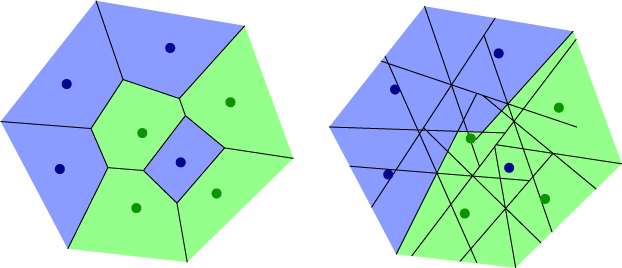
\includegraphics[width=0.9\textwidth]{knn1}
\label{fig:knn1}  

\end{figure}

\subsection{Árvore de Decisão}



Em sua forma mais simples, árvores de decisão são uma classe de algoritmos que buscam (no caso de classificação) achar a classe de um ponto de treino testando intervalos de suas \textit{features}. Vejamos o exemplo de uma árvore treinada a seguir:


\begin{figure}[ht]
	\centering
	\caption{Árvore de Decisão para prever a sobrevivência de passageiros do Titanic}
  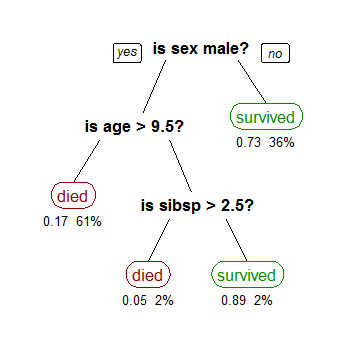
\includegraphics[width=0.9\textwidth]{tree1}
\label{fig:tree1}  

\end{figure}

Essa árvore busca prever se um determinado passageiro do Titanic sobreviveu ou não ao acidente testando diversas características desse indivíduo. Por exemplo, podemos ver que caso o sexo do passageiro seja feminino, ela tem uma alta chance de ter sobrevivido. Caso contrário, já são testadas outras duas cláusulas referentes a idade ao número de familiares também a bordo do navio. Por construção, temos um \textit{trade-off} para árvores, podendo trocar \textbf{legibilidade} por \textbf{precisão} (menos \textit{bias}). É possível construir árvores mais complexas que poderão a sua facilidade de interpretação por uma pessoa, porém poderão se adequar melhor ao dados treinados, e é essa ideia que é explorada por algoritmos de \textit{ensemble learning} como \textit{Random Forests} ou \textit{Adaboost}, que serão explicados em outra parte desse documento, mas que basicamente combinam o poder de diversas árvores treinadas iterativamente, para aumentar seu poder de classificação.


\subsection{Support Vector Machines}

Essa classe de algoritmos busca, para um conjunto de dados N-dimensionais, encontrar um hiperplano que separa o espaço dos dados em regiões de classificação. Vejamos um exemplo simples a seguir:


\begin{figure}[ht]
	\centering
	\caption{SVM aplicado para classificar dados linearmente separáveis}
  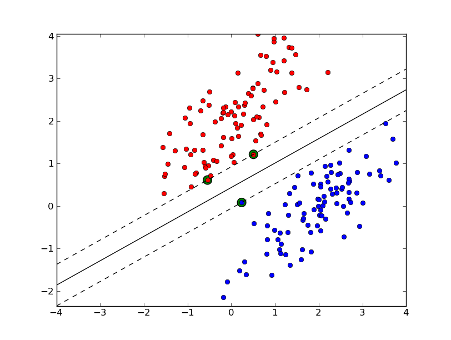
\includegraphics[width=0.9\textwidth]{svm1}
\label{fig:svm1}  

\end{figure}



A reta na imagem foi encontrada de modo a separar o espaço de classificação da classe "azul" do espaço de classificação da classe "vermelha". A linha pontilhada representa a margem de classificação, o algoritmo busca chegar a um hiperplano que tenha ainda uma distância dos pontos mais próximos da região de separação. A seguir, um exemplo mais complexo usando um \textit{kernel}  para poder classificar dados não linearmente separáveis:

\begin{figure}[ht]
	\centering
	\caption{SVM aplicado para classificar dados de maneira não linear}
  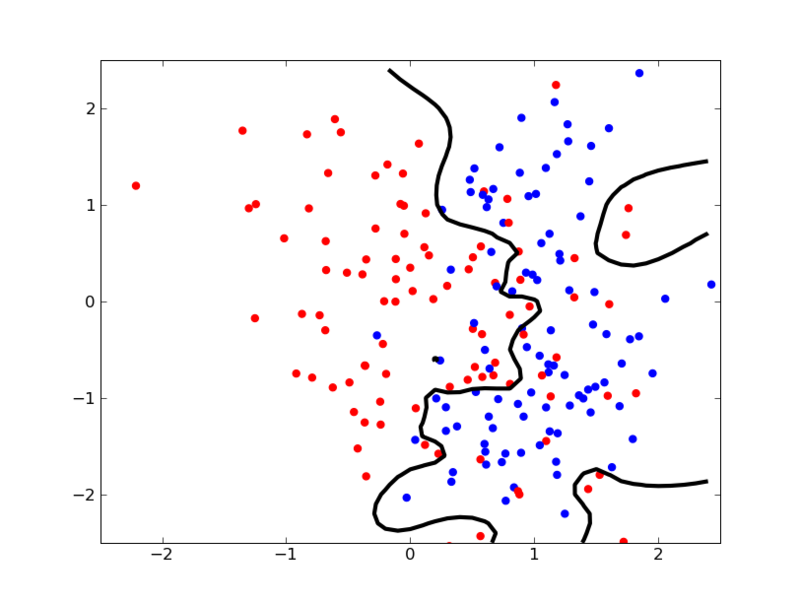
\includegraphics[width=0.9\textwidth]{svm2}
\label{fig:svm2}  

\end{figure}



\chapter{Especificação}\label{chp:espec}
\section{Requisitos}\label{sec:req}

\subsection{Requisitos Funcionais}
- Enviar dados sobre a intensidade dos sinais de \textit{Wi-fi} ao servidor. \par
- Retornar a posição do usuário baseado nos dados enviados.\par
- Disponibilizar uma API para ser usada por outras aplicações.\par


\subsection{Requisitos Não-Funcionais}

- O sistema deve ser transparente ao usuário.\par

\section{Pontos de Vista}\label{sec:viewpoints}
\subsection{Ponto de Vista da Empresa}
Este projeto deverá criar um sistema de localização precisa em ambientes fechados, utilizando como parâmetros as intensidades de sinais redes sem fio próximas. O resultado deste projeto incluirá duas aplicações:\par
Aplicativo para o celular com dois módulos utilizados para capturar informações das redes sem fio próximas e enviá-las servidor, além de receber resultados deste servidor e exibi-los para o usuário;\par
Aplicação em nuvem que receberá os dados dos celulares e responderá com a localização do usuário.\par
Para tal serão feitas análises estatísticas do comportamento e flutuação do sinal de \textit{Wi-fi} em diversas medições e com aparelhos de celular diferentes e posteriormente, estes dados serão analisados por um algoritmo de inteligência artificial baseado em \textit{machine learning}, para que a localização seja definida.
\subsection{Ponto de Vista da Informação}
As informações processadas pelo sistema seguirão dois fluxos. No primeiro as intensidades dos sinais provenientes dos pontos de acesso de redes sem fio serão capturadas pelo sensor do celular e registradas pelo módulo de aquisição de dados do aplicativo. Em seguida, estas informações serão enviadas para o servidor para que recebam o devido tratamento.\par
Após o período de treinamento do sistema o segundo fluxo será possível. Nele após o dispositivo móvel enviar os sinais capturados por um usuário regular, o servidor deve executar seu algoritmo de \textit{machine learning} e retornar à posição que o usuário se encontra dentro do prédio previamente estabelecido, usando como base estes dados enviados.\par
A troca de dados em ambos os fluxos será feita usando o formato JSON, este formato é muito utilizado principalmente quando é necessária a implementação de tabelas de bancos de dados por conta de sua simplicidade para manipular as informações representadas.
\subsection{Ponto de Vista da Computação}
O sistema será composto por duas partes funcionais, a primeira é o aplicativo desenvolvido para dispositivos Android, ele será responsável pela captura dos dados, em seguida ele organizará as informações coletas no formato JSON e finalmente realizará a transmissão por meio da rede à qual o dispositivo estiver conectado, uma rede 3G/4G ou pela conexão a uma rede \textit{Wi-fi} disponível.\par
A segunda parte é o servidor em nuvem, que deverá processar os dados executando o algoritmo de \textit{machine learning} e em seguida disponibilizará os resultados obtidos para posterior consulta feita quando forem requisitadas informações a respeito do ambiente fechado já mapeado anteriormente, retornando a posição do usuário.
\subsection{Ponto de Vista da Engenharia}
Para o uso do sistema será necessário que o dispositivo móvel que executar o aplicativo tenha uma antena de \textit{Wi-fi}, para que possam ser realizadas as medições de intensidades dos sinais. Tais dados serão enviados pela própria antena de \textit{Wi-fi} usando a rede que estiver conectada ou pela antena de 3G/4G usando as redes móveis para o servidor. O serviço funcionará em uma máquina virtual hospedada no serviço Amazon AWS, sendo que esta máquina deverá ser capaz de execução do algoritmo de \textit{machine learning}.\par
É necessário também que exista uma estrutura mínima no local a ser mapeado, deve existir um número mínimo de pontos de acesso de rede sem fio suficiente para englobar todo o ambiente. Esta cobertura não deve ser apenas de pelo menos um sinal \textit{Wi-fi} na parcela de área, é indispensável que mais de um sinal atinja cada ponto para que seja possível haver a determinação do ponto escolhido.
\subsection{Ponto de Vista da Tecnologia}
O processamento e aplicação dos algoritmos de \textit{machine learning} serão feitos por meio da linguagem R. O aplicativo é feito para a plataforma Android e o servidor é implementado na plataforma \textit{Ruby on Rails}, hosteado em servidor Amazon AWS, para pequenas aplicações que devem rodar na nuvem. O R é servido por meio de uma plataforma REST por meio da biblioteca Plumber, que permite que chamadas as funções do R sejam feitas por meio de requisições HTTP.

\chapter{Metodologia}

\section{Gerenciamento de tarefas}
O projeto desde a sua idealização foi gerenciado com metodologia \textit{Kanbam}, com a equipe sempre desenvolvendo \textit{features} incrementais com pequenos protótipos entregáveis. A ferramenta de gestão utilizada pelo grupo foi o Trello, aplicação de gerenciamento de projetos baseado na web. Foi sempre feita a distinção entre pesquisa, documentação e implementação. Como é típico de metodologias ágeis, os testes sempre foram realizados em paralelo com a implementação de cada nova \textit{feature}, de modo que para cada nova parte do projeto implementada, foram realizados testes para garantir que as funções antigas ainda funcionam individualmente.
\section{Gerenciamento de código}
Para hospedar e versionar os códigos-fonte dos programas foram utilizados repositórios do GitHub, serviço Git baseado em nuvem, gratuito para \textit{softwares Open-Source}. O Git consiste num sistema de controle de versão de software distribuído, com objetivo de minimizar conflitos entre códigos de diferentes contribuidores em um mesmo repositório.

\section{Pesquisa} 
A pesquisa foi feita concomitantemente com todo o desenvolvimento dos \textit{sprints}, com novas possibilidades sendo estudadas e implementadas as vezes ao mesmo tempo. Foram de vital importância as ideias tiradas de \textit{papers} nas partes de \textit{ensemble learning} \cite{comparativeEN}, normalização e tratamentos dos dados, bem como a estrutura dos testes de \textit{cross validation} \cite{comparative}, e também na fundamentação teórica do método \textit{Adaboost} \cite{explainingadaboost} e \cite{adaboost}.
\chapter{Projeto e Implementação}\label{chp:ml}


\section{Tratamento dos dados}\label{sec:data1}

\subsection{Dados obtidos do Repositório UCI}
	Para grande parte dos testes de \textit{cross-validation}, foi usado o \textit{dataset}  \textit{UJIIndoorLoc} apresentado em \cite{uji}. O \textit{dataset} consiste em diversas medidas de potência de sinal \textit{Wi-fi} medidas com diversos aparelhos celulares em 3 prédios diferentes de uma faculdade. As medidas estão separadas por prédio, andar e sala. Para os fins dessa monografia, serão realizados testes com medidas sempre de um mesmo andar, afim de classificar as zonas de um mesmo ambiente.  Esse  \textit{dataset} usa a constante $100$ para designar valores não medidos. Para começar o tratamento os substituímos pelo valor de $-120$ (dB), que para todos os fins práticos, é uma medida de potência que representa um valor nulo, já que representa um valor de potência insignificante. E finalmente, antes de serem usados para treinar os modelos, os dados são transformados de modo a ficarem com média 0 e variância 1 por coluna, o que é necessário para evitar comportamentos indesejados dos algoritmos de ML.

A transformação é realizada da seguinte maneira, com $X_j$ representando a j-ésima coluna da matriz de dados, com média $\mu$ e desvio-padrão $\sigma$, para cada elemento $i$ dessa coluna:

\begin{center}
$X_{ij}=\frac{X_{ij}-\mu}{\sigma}$
\end{center}

\subsection{Dados do Servidor}

De modo análogo aos dados pegos do Repositório UCI, a matriz de dados é transformada para ter média nula e variância unitária em cada coluna, sendo que antes disso valores nulos são substituídos por $-120$.




\section{Formato dos dados tratados}
A matriz de dados, depois de tratada, tem o seguinte formato:

\begin{center}
\begin{blockarray}{cccccc}
$ZoneID$ & $BSSID_1$ & $BSSID_2$ & ... &  $BSSID_n$ \\
\begin{block}{(ccccc)c}
  1&-70 & -92 &   ... &-87&  $ Measure_1$ \\
  2&-89 & -80 & ... & -63&    $Measure_2 $\\
  3&-28 & -120 & ...&   -35& $Measure_3$ \\
   \vdots& \vdots &  \vdots & $\ddots$ &  \vdots &    \vdots \\
  1&-48 & -36 & ... &   -29&  $Measure_n$ \\
\end{block}
\end{blockarray}
\end{center}

Cada coluna representa a medida de uma \textit{BSSID} (i.e. um Roteador), ou seja, uma \textit{feature} para o ML, e cada linha é um ponto de treino (i.e.  uma medida para cada  \textit{BSSID}, nossas \textit{features}).


\section{Modelos Usados e \textit{Cross-Validation} de parâmetros }

A chamada \textit{cross-validation} dos modelos de ML é o teste para encontrar os parâmetros ótimos para o treinamento. Um dos métodos escolhidos de \textit{cross-validation} foi o \textit{k-fold}. O método \textit{k-fold} divide o dataset em $K$ subconjuntos de igual tamanho e então um dos conjuntos é usado como validação do treinamento feito pelos $K-1$ subconjuntos restantes. O processo é repetido $K$ vezes e em cada subdivisão possível podem ser usados valores de parâmetros de treino distintos. Para a comparação dos modelos, serão feitos diversos testes com um número crescente de zonas de classificação. Nesse caso, são escolhidas iterativamente e aleatoriamente $n$ zonas do \textit{dataset}  \textit{UJIIndoorLoc}, são pegos todos os pontos associados as $n$ zonas selecionadas. Então, o \textit{dataset}  é separado em 80\% de pontos de treino e 20\% para testes. Para valores de $n$ de 1 a 30 são finalmente medidos as taxas de erro de cada algoritmo e essa informação é apresentada em gráficos.

\subsection{KNN : K-Nearest-Neighbors }


Para o algoritmo de KNN, foram feitos dois testes de \textit{cross-validation}. No primeiro, a métrica de distância foi decidida, e no segundo, o número de vizinhos ($K$).
Para que fosse definida a métrica de distância, foi usado o método  \textit{k-fold}  com $K=2$. E em cada \textit{fold} o modelo foi treinado com uma métrica diferente. Foram calculados 20 conjuntos diferentes de \textit{folds} e foi tirada a média do erro de validação para cada uma das métricas.


\begin{figure}[H]
\centering
\caption{Erros para uso de Diferentes Distâncias}
 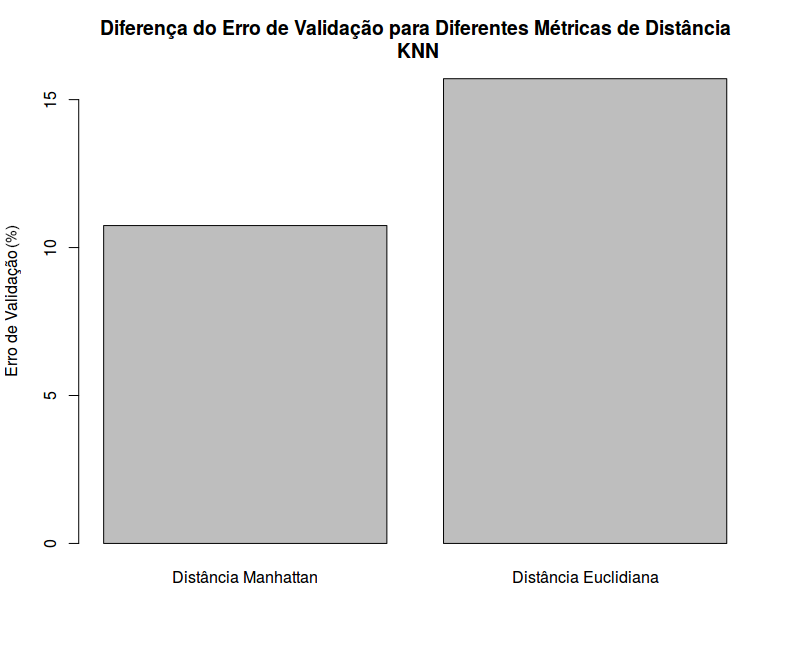
\includegraphics[width=0.9\textwidth]{euclidianManhattanknn21zonas}
\label{fig:euclidian}
\end{figure}


Depois, foi usado o método  \textit{k-fold} com $K=10$ para a decisão do número de vizinhos. Foram testados os valores de 1 até 10 para o número de vizinhos. Na imagem a seguir vemos detalhes desse teste.


\begin{figure}[H]
\centering
\caption{Erro em função do número de vizinhos}
 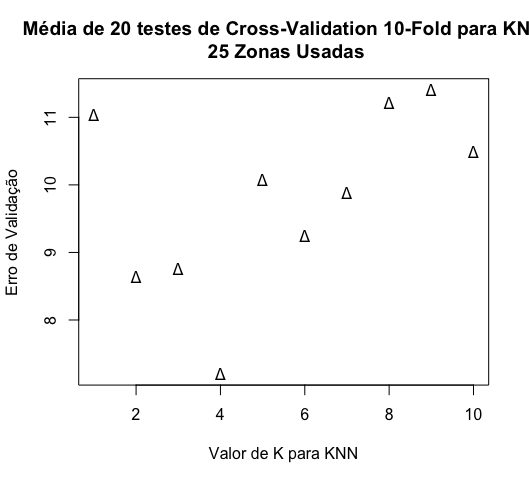
\includegraphics[width=0.9\textwidth]{CrossValKNN25zonasvalorK}
\label{fig:crossValKNN}
\end{figure}



Podemos concluir então que (1) o erro é menor no geral com a distância de \textit{Manhattan} e (2) embora tenha muita variância envolvida no teste, o valor de K que minimiza o erro fica proximo de 4 vizinhos.


No restante do trabalho foi escolhido o valor de $K=4$ vizinhos.



\subsection{Rede Neural}

Para a \textit{cross-validation} das Redes Neurais, também foi usado o método de  \textit{k-fold} com $K=10$. Para cada uns dos\textit{folds} foi testado um número de neurônios em uma  \textit{hidden-layer} única. (Outros testes mostraram não valer a pena para o nosso problema usar mais de uma camada de  \textit{hidden layer} ou \textit{deep learning}). Os resultados são mostrados a seguir:



\begin{figure}[H]
	\centering
	\caption{Erro para diversas quantidades de neurônios na rede neural.}
  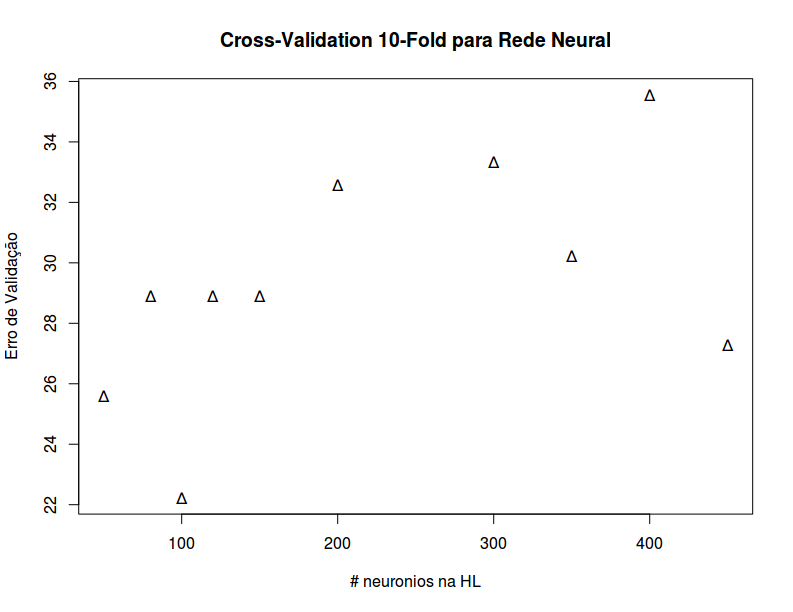
\includegraphics[width=0.9\textwidth]{CROSSVALE4ZonasNNCERTO}
\label{fig:crossNN}

\end{figure}




Concluímos que o número ideal de neurônios na  \textit{hidden-layer} está próximo de 200. Porém, com estudos e testes mais detalhados ficou claro que as Redes Neurais não são ideias para o nosso projeto, por não conseguirem capturar de forma satisfatória o modelo do nosso problema. Além disso, o algoritmo de \textit{back propagation} se mostra muito mais custoso em relação a memória e processamento se comparado aos outros algoritmos usados no projeto, demorando cerca de 10 vezes mais para o treinamento que todos os outros modelos juntos. Portanto, seu uso foi descartado.

\subsection{Arvore de decisão}


Baseado no trabalho apresentado por \cite{comparative}, foi escolhida uma implementação do algoritmo C4.5 \cite{quinlan} em Java, da biblioteca Weka, para serem geradas árvores de decisão. Os métodos porém foram chamados pela interface da Weka para R, chamada RWeka.
A função J48 do Weka foi testada com o os pontos de treino referentes ao primeiro andar do prédio 1 (i.e. BuildingID 1, FloorID 0)  do dataset \textit{UJIIndoorLoc}. Foi levantada a curva de erro de classificação para uma quantidade crescente de pontos de treino (como explicado em 2.3).


\begin{figure}[H]
\centering
\caption{Teste de Validação do Algoritmo C4.5}
 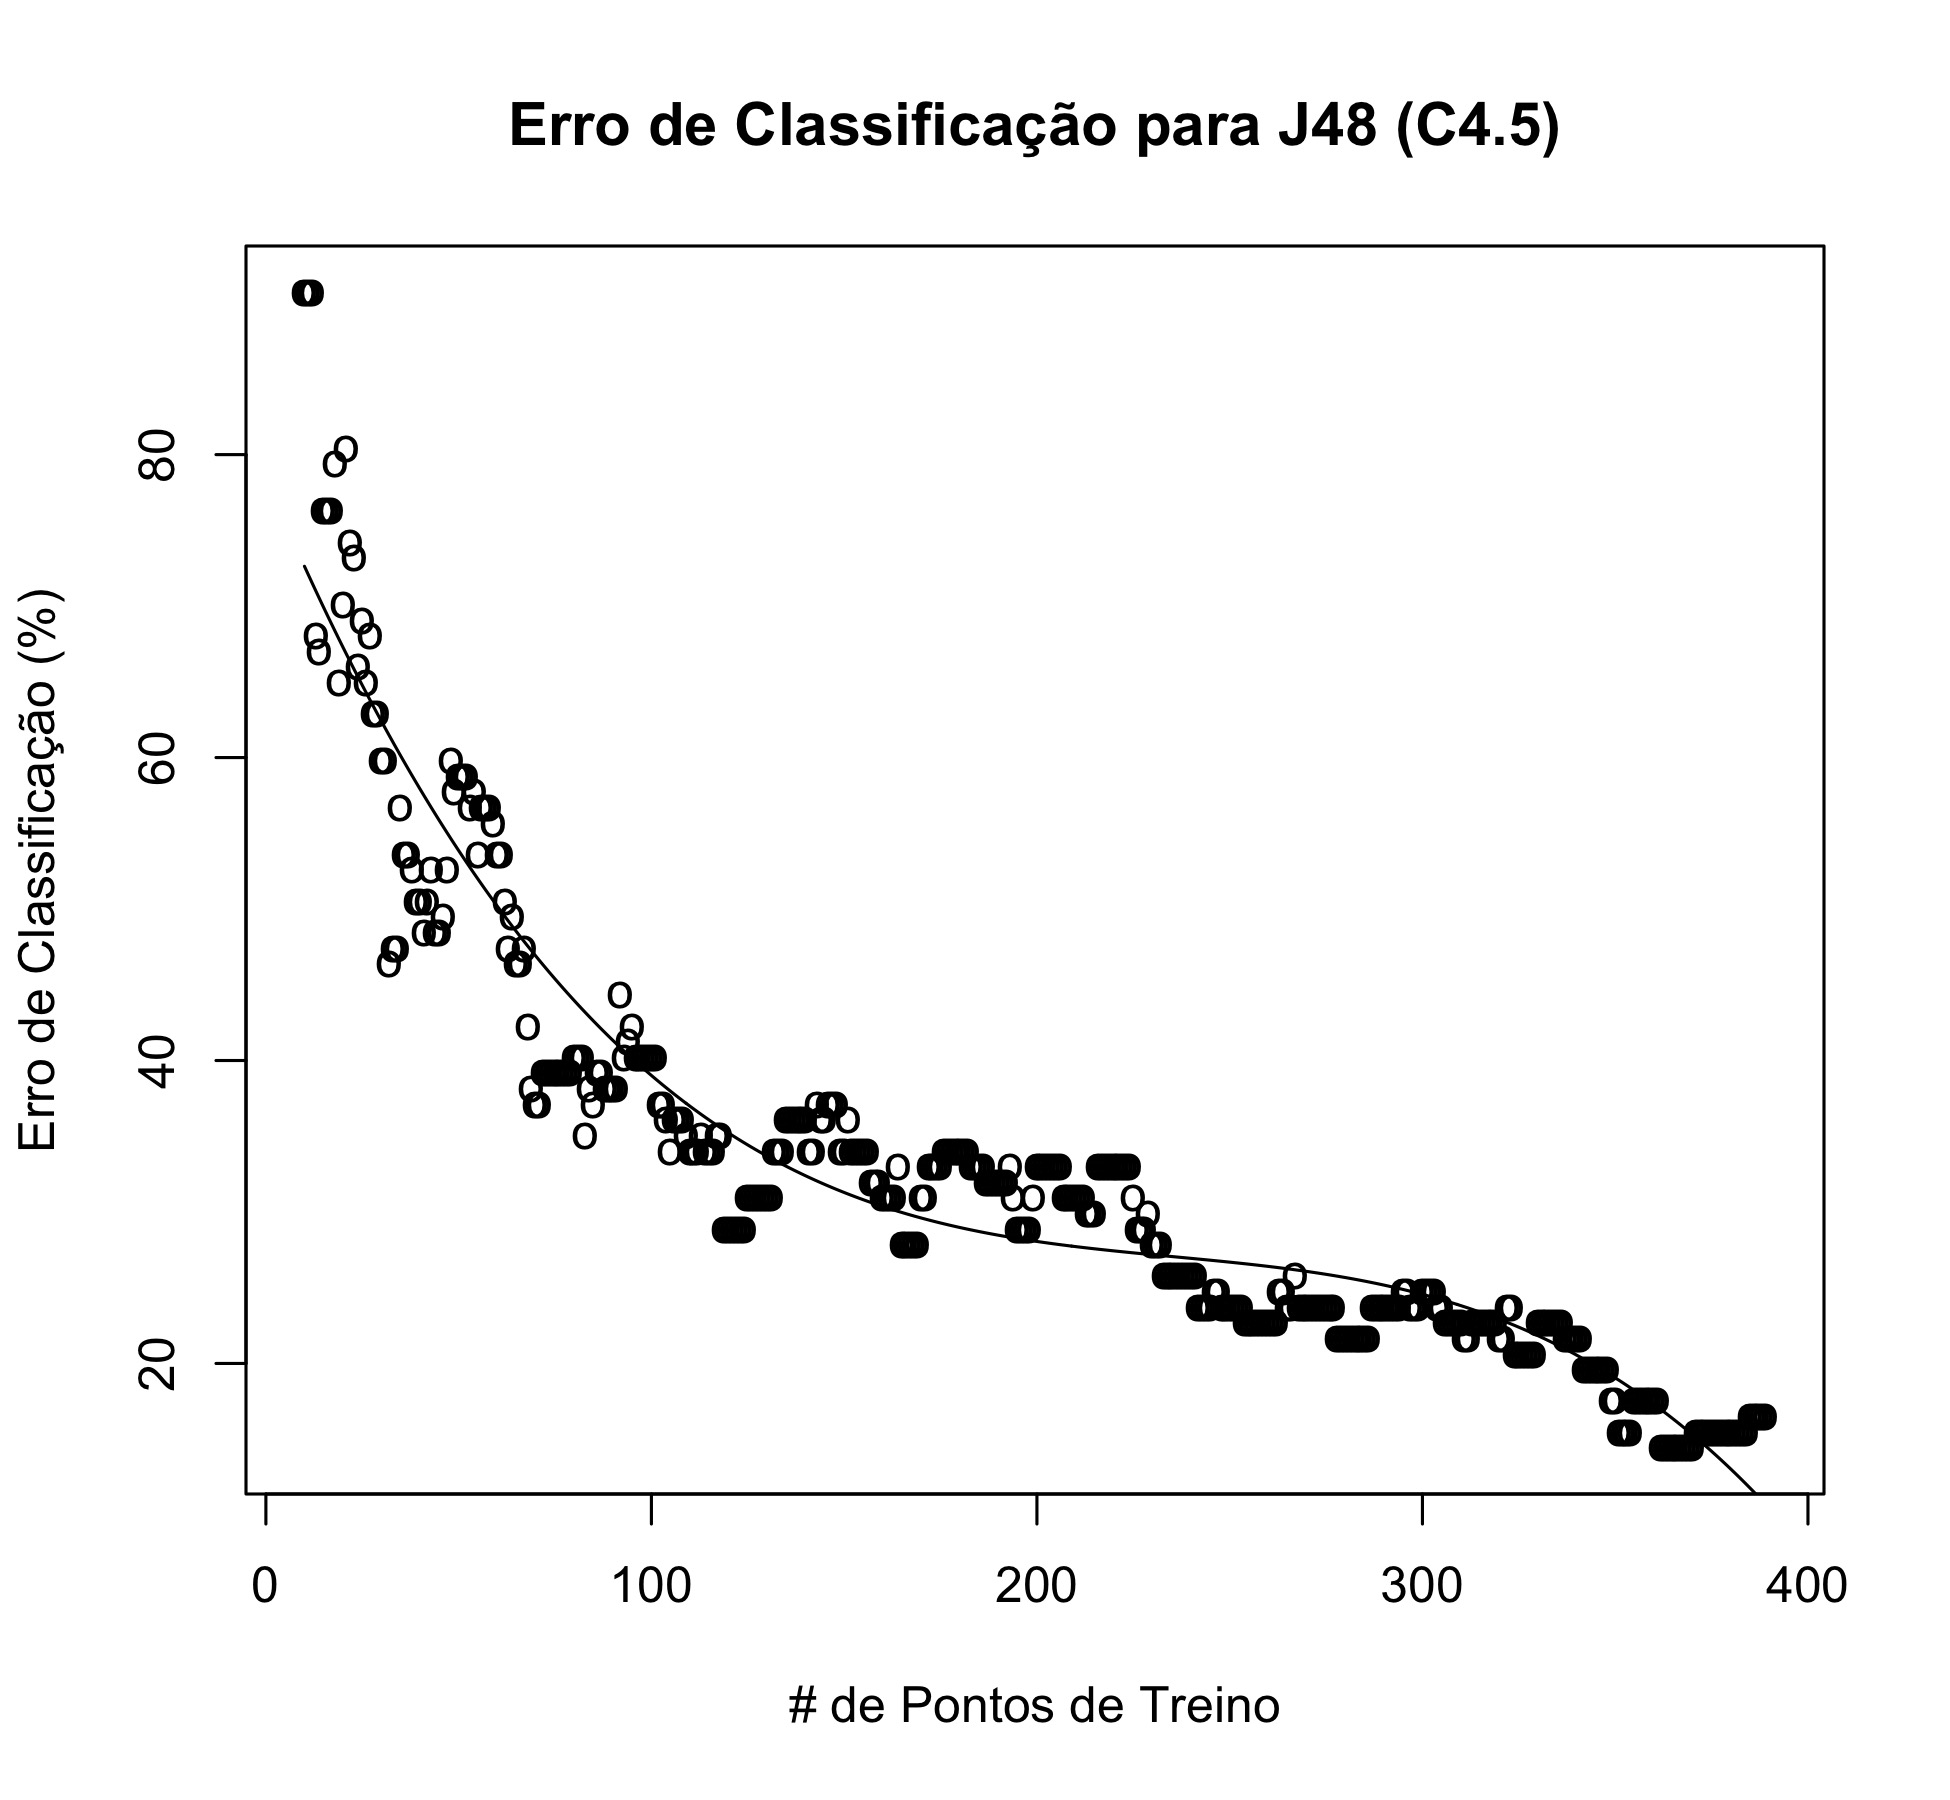
\includegraphics[width=0.9\textwidth]{J48Validacaopredio1andar0}
\label{fig:validationC4.5}
\end{figure}

\subsubsection{Acoplamento com o Algoritmo AdaBoost}




\textit{Boosting} é a ideia em ML de criar uma predição forte e precisa combinando diversas previsões mais fracas. O algoritmo AdaBoost \cite{adaboost} é um método para melhorar a precisão de classificadores fracos (i.e. \textit{Weak Learners}) por meio de uma votação ponderada que leva em conta o erro de diversos votadores fracos treinados no processo. É provado que o modelo final se torna um classificador forte \cite{explainingadaboost}. Por definição, um classificador fraco é aquele que consistentemente consegue ser melhor que um chute para a classificação (e.g. o erro é menor que 50\% para o caso de duas classes possíveis de classificação).

Também baseados em \cite{comparative} e \cite{comparativeEN}. Usaremos o algoritmo AdaBoost  e sua implementação na biblioteca Weka para melhorar a precisão das árvores de decisão C4.5. A seguir vemos um gráfico comparando a classificação para o mesmo andar do \textit{dataset UJIIndoorLoc} com os mesmos pontos de teste e uma quantidade crescente de pontos de treino, assim como feito no tópico anterior.


\begin{figure}[!h]
\centering
\caption{Comparação do C4.5 com o uso do AdaBoost}
 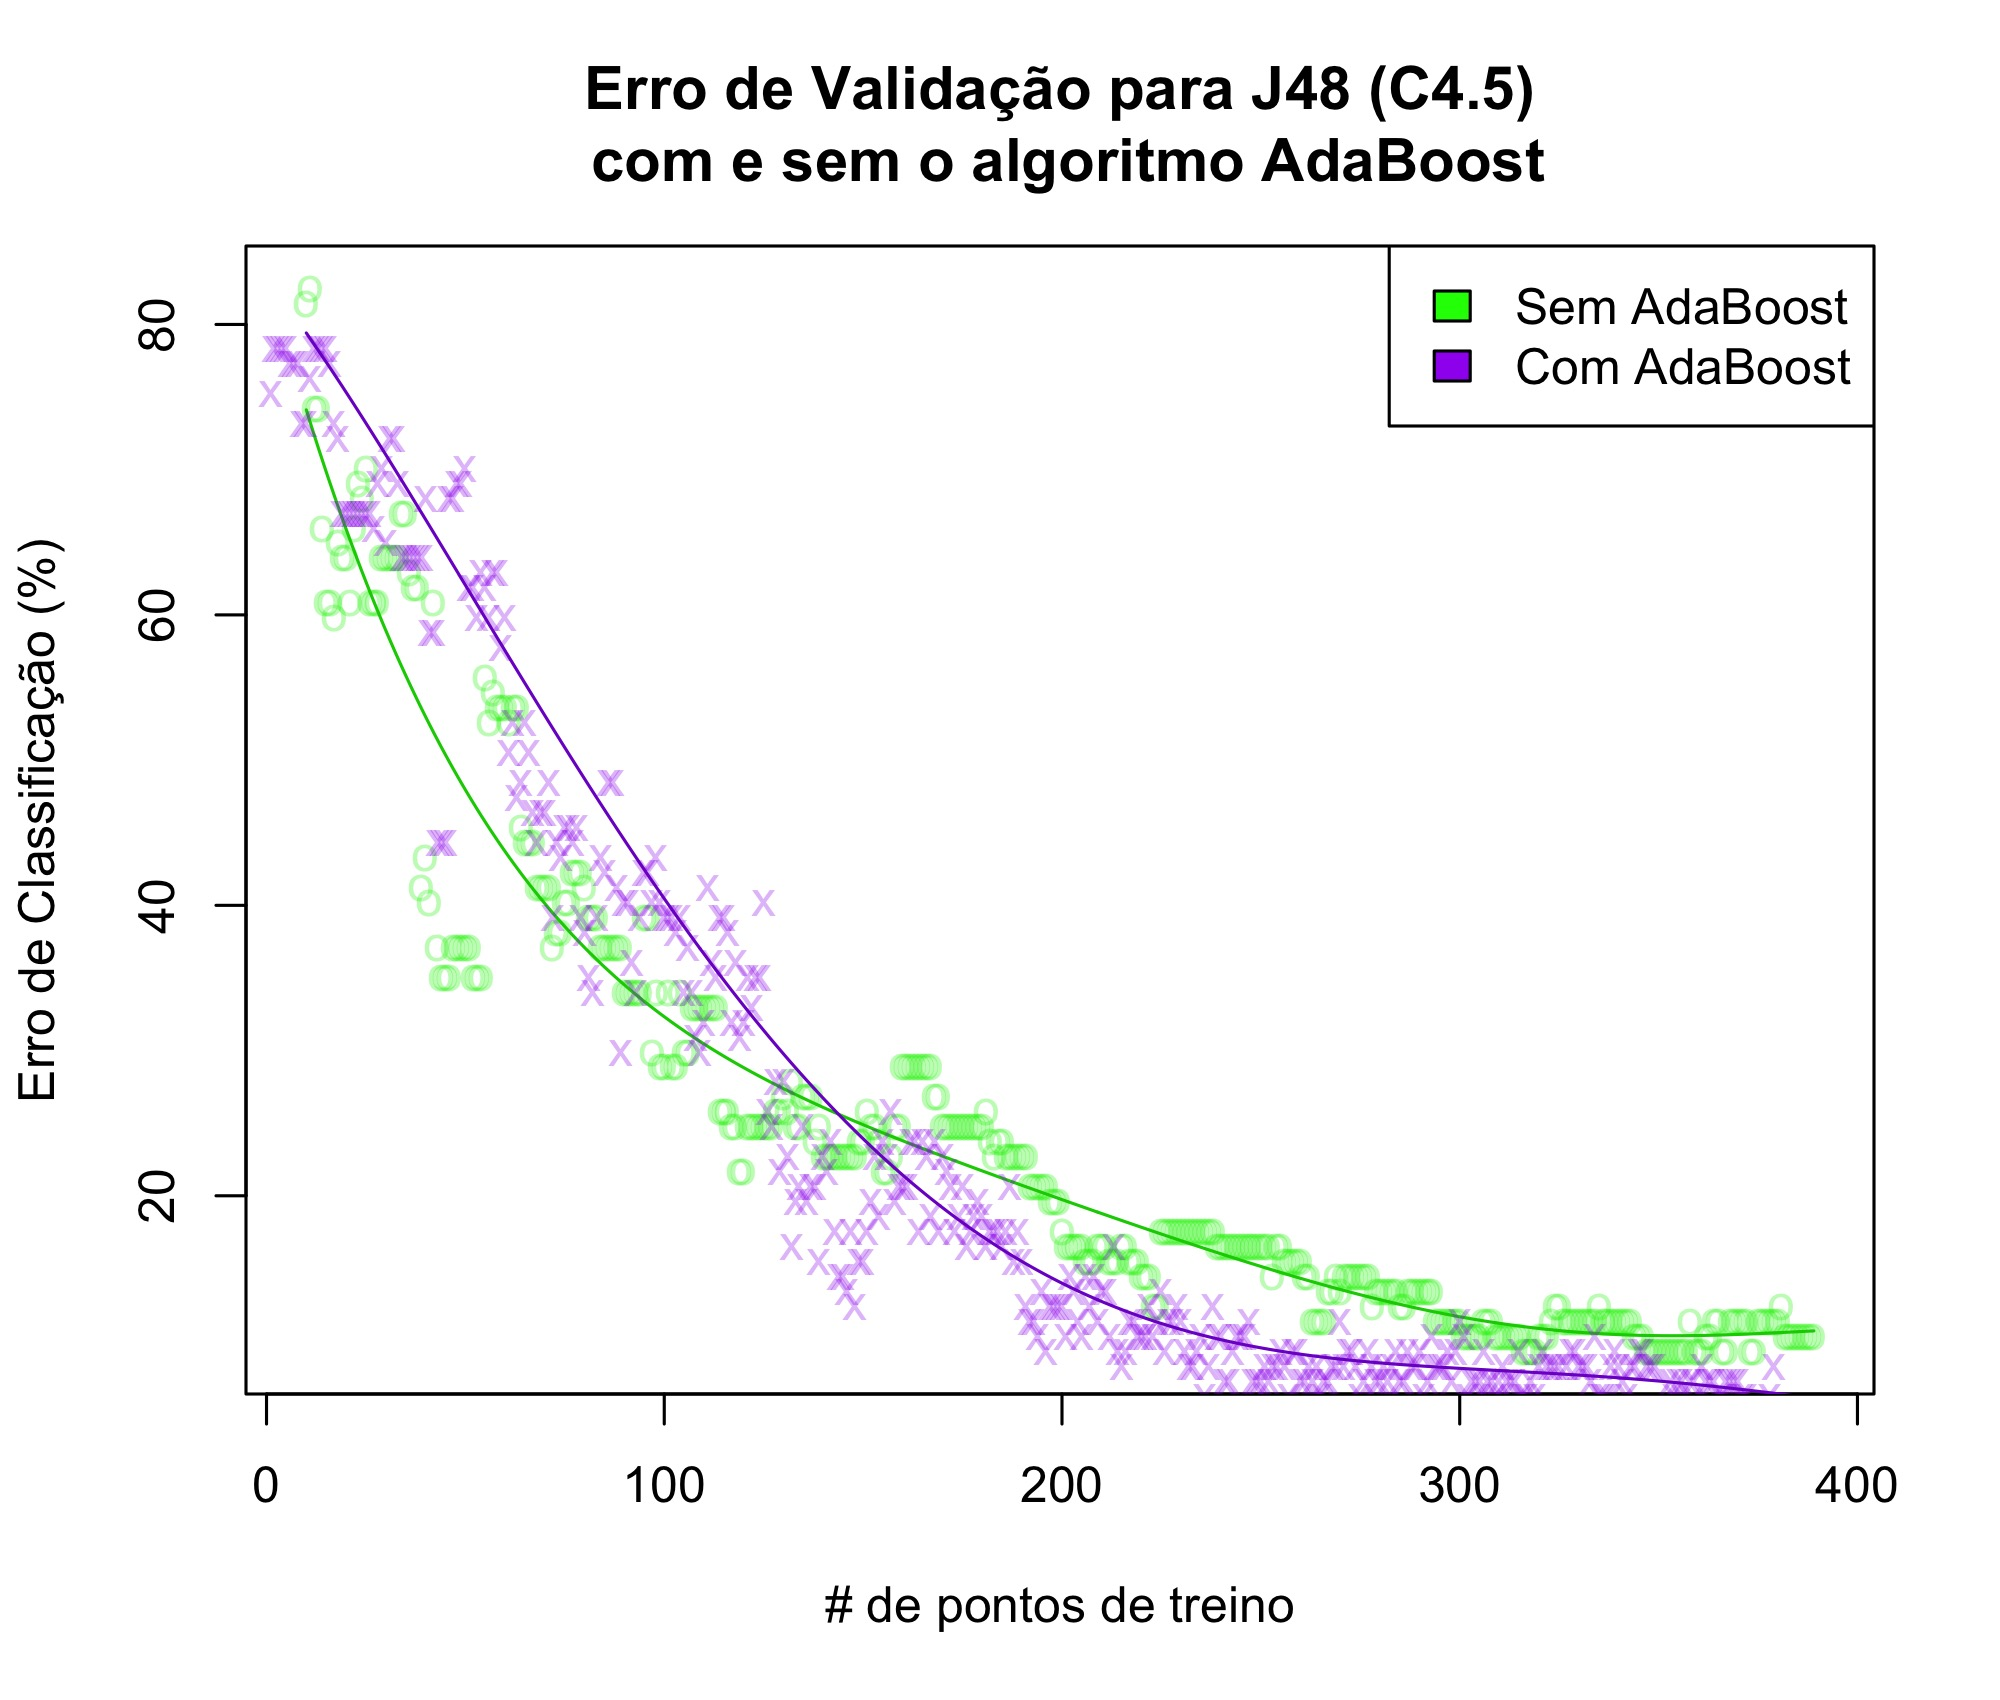
\includegraphics[width=0.9\textwidth]{J48xADAValidacaopredio1andar0}
\label{fig:comparisonC4.5andAdaBoost}  
\end{figure}


Podemos notar que com um número grande de pontos de treino, obtemos uma melhora sensível de precisão para a classificação, e portanto, no restante do trabalho, iremos usar o algoritmo C4.5 acoplado com o algoritmo AdaBoost.



\subsection{Comparação dos Modelos Usados}


Reiterando o que foi explicado em outra sessão, os testes a seguir irão contemplar todos os modelos usados. Os modelos tem seu erro testado para \textit{datasets} com um número crescente de zonas aleatórias a serem classificadas. Todos os testes foram feitos com os dados do primeiro andar do prédio 1 do \textit{dataset UJIIndoorLoc }(i.e. BuildingID 1, FloorID 0).


\begin{figure}[!h]
	\centering
	\caption{Erro do algoritmo SMO  para uma quantidade crescente de zonas de classificação.}
  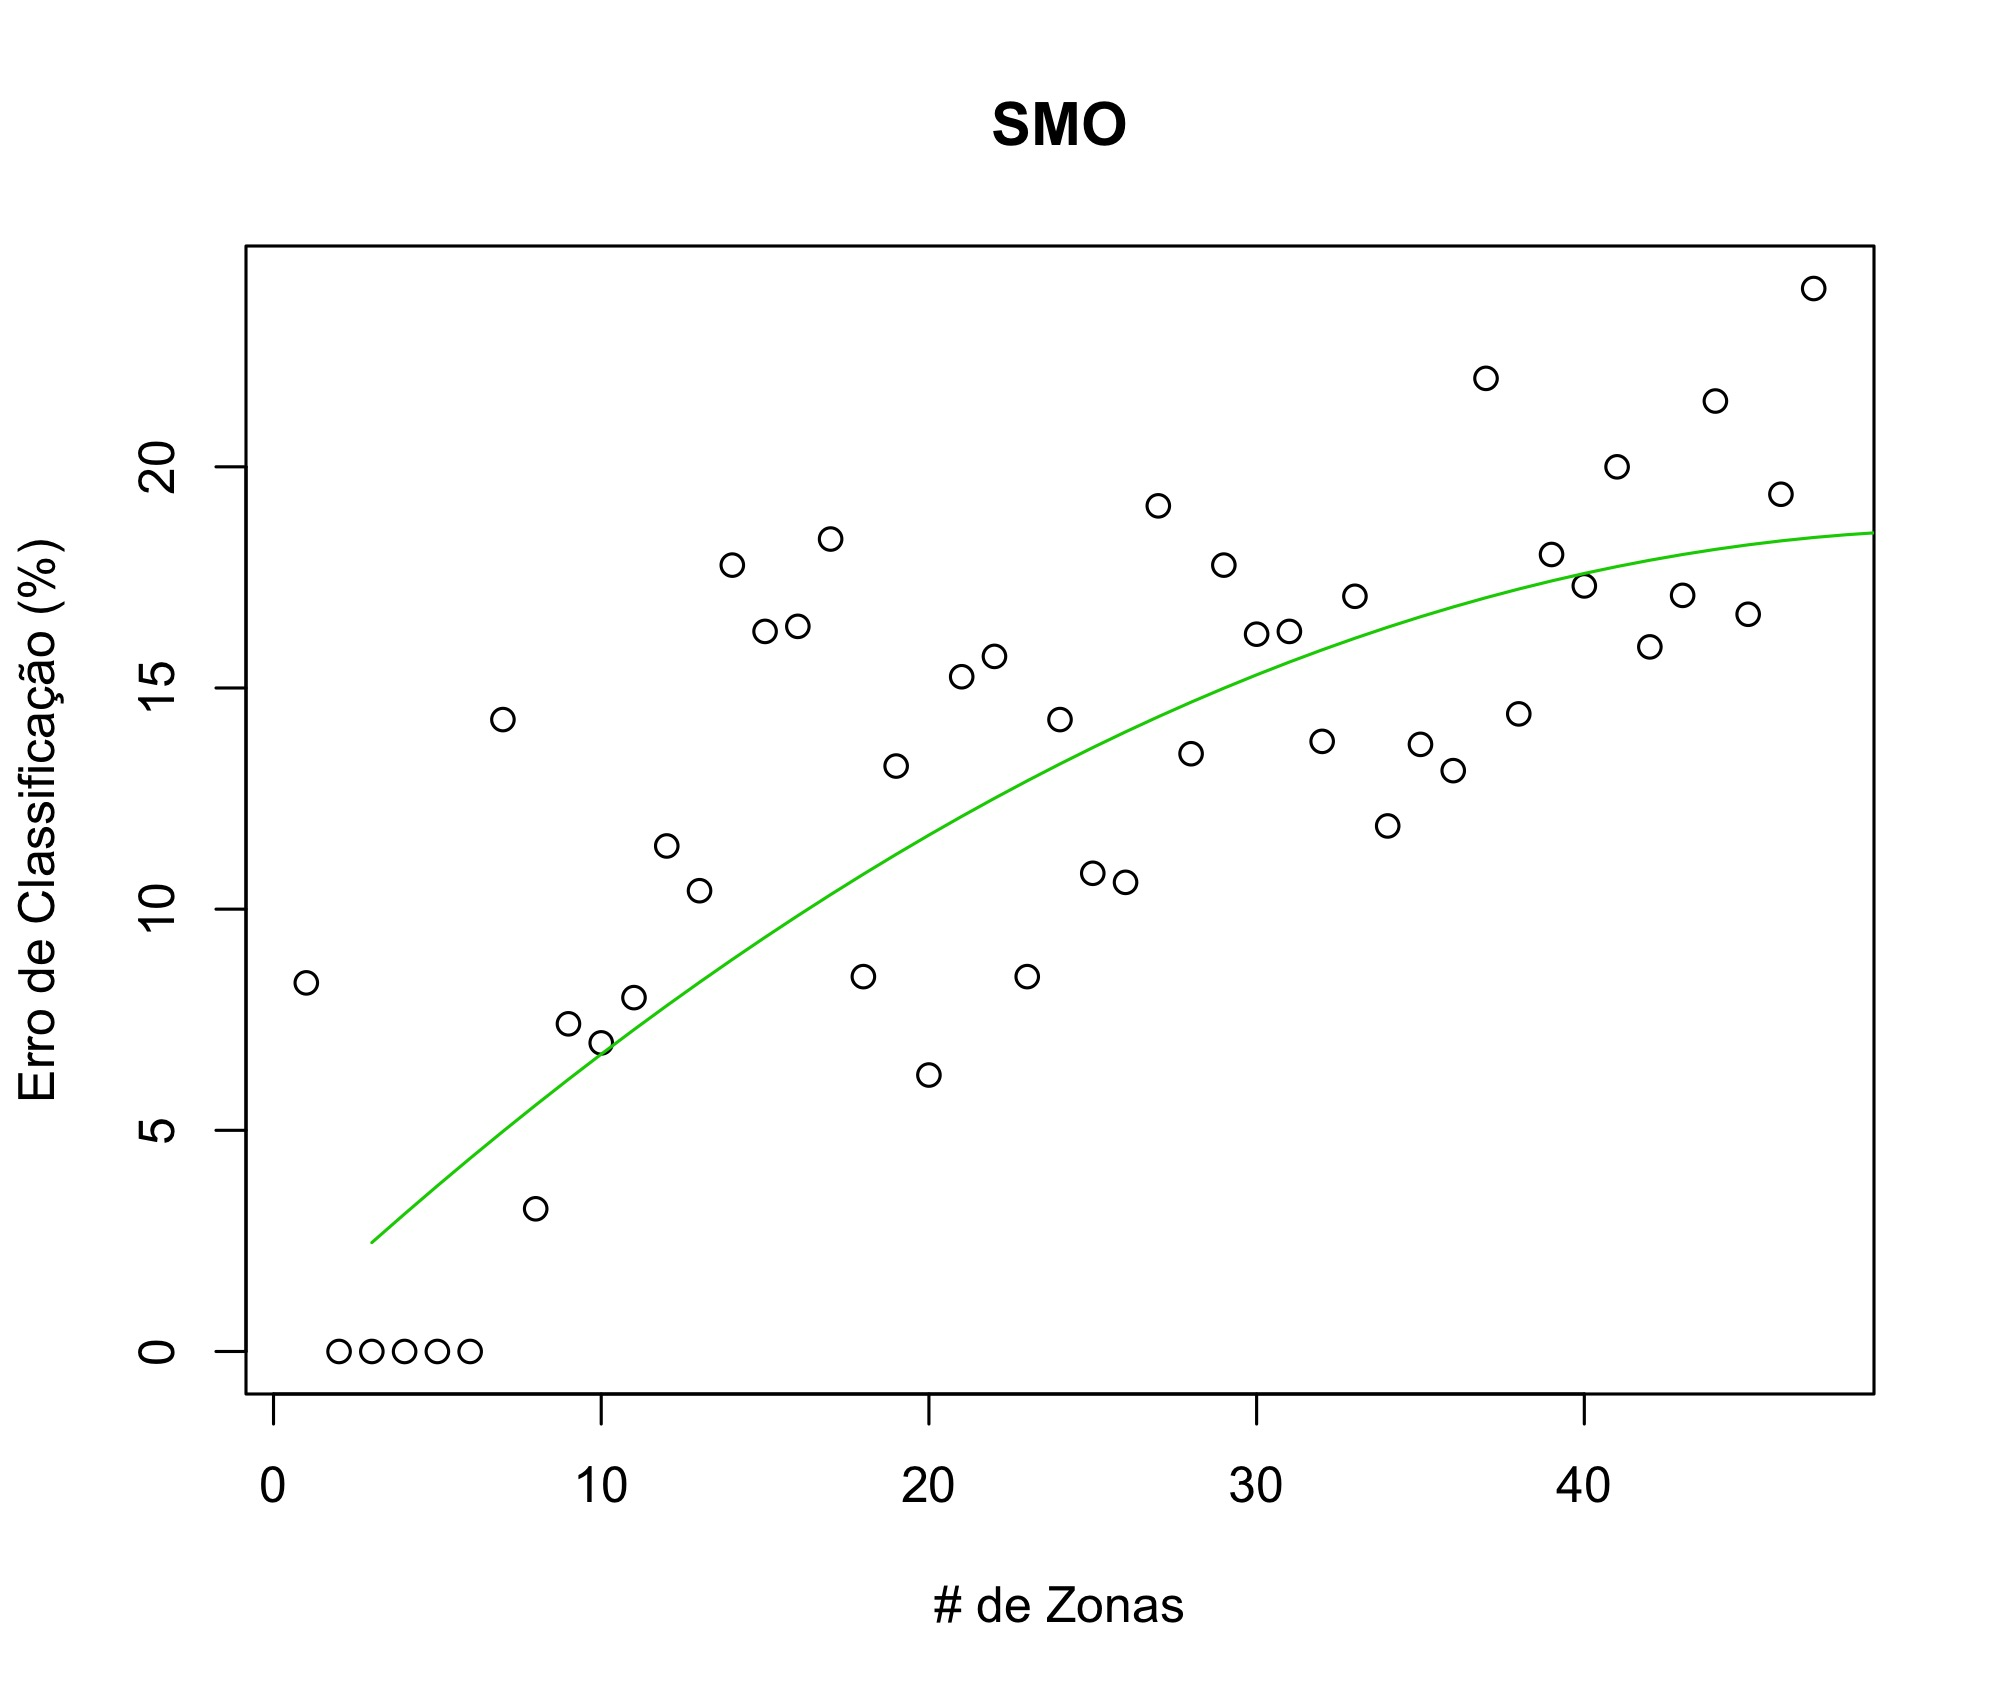
\includegraphics[width=0.9\textwidth]{errorporzonaSMO}
\label{fig:zonaSMO}

\end{figure}



\begin{figure}[!h]
	\centering
	\caption{Erro do algoritmo de Redes Neurais  para uma quantidade crescente de zonas de classificação.}
  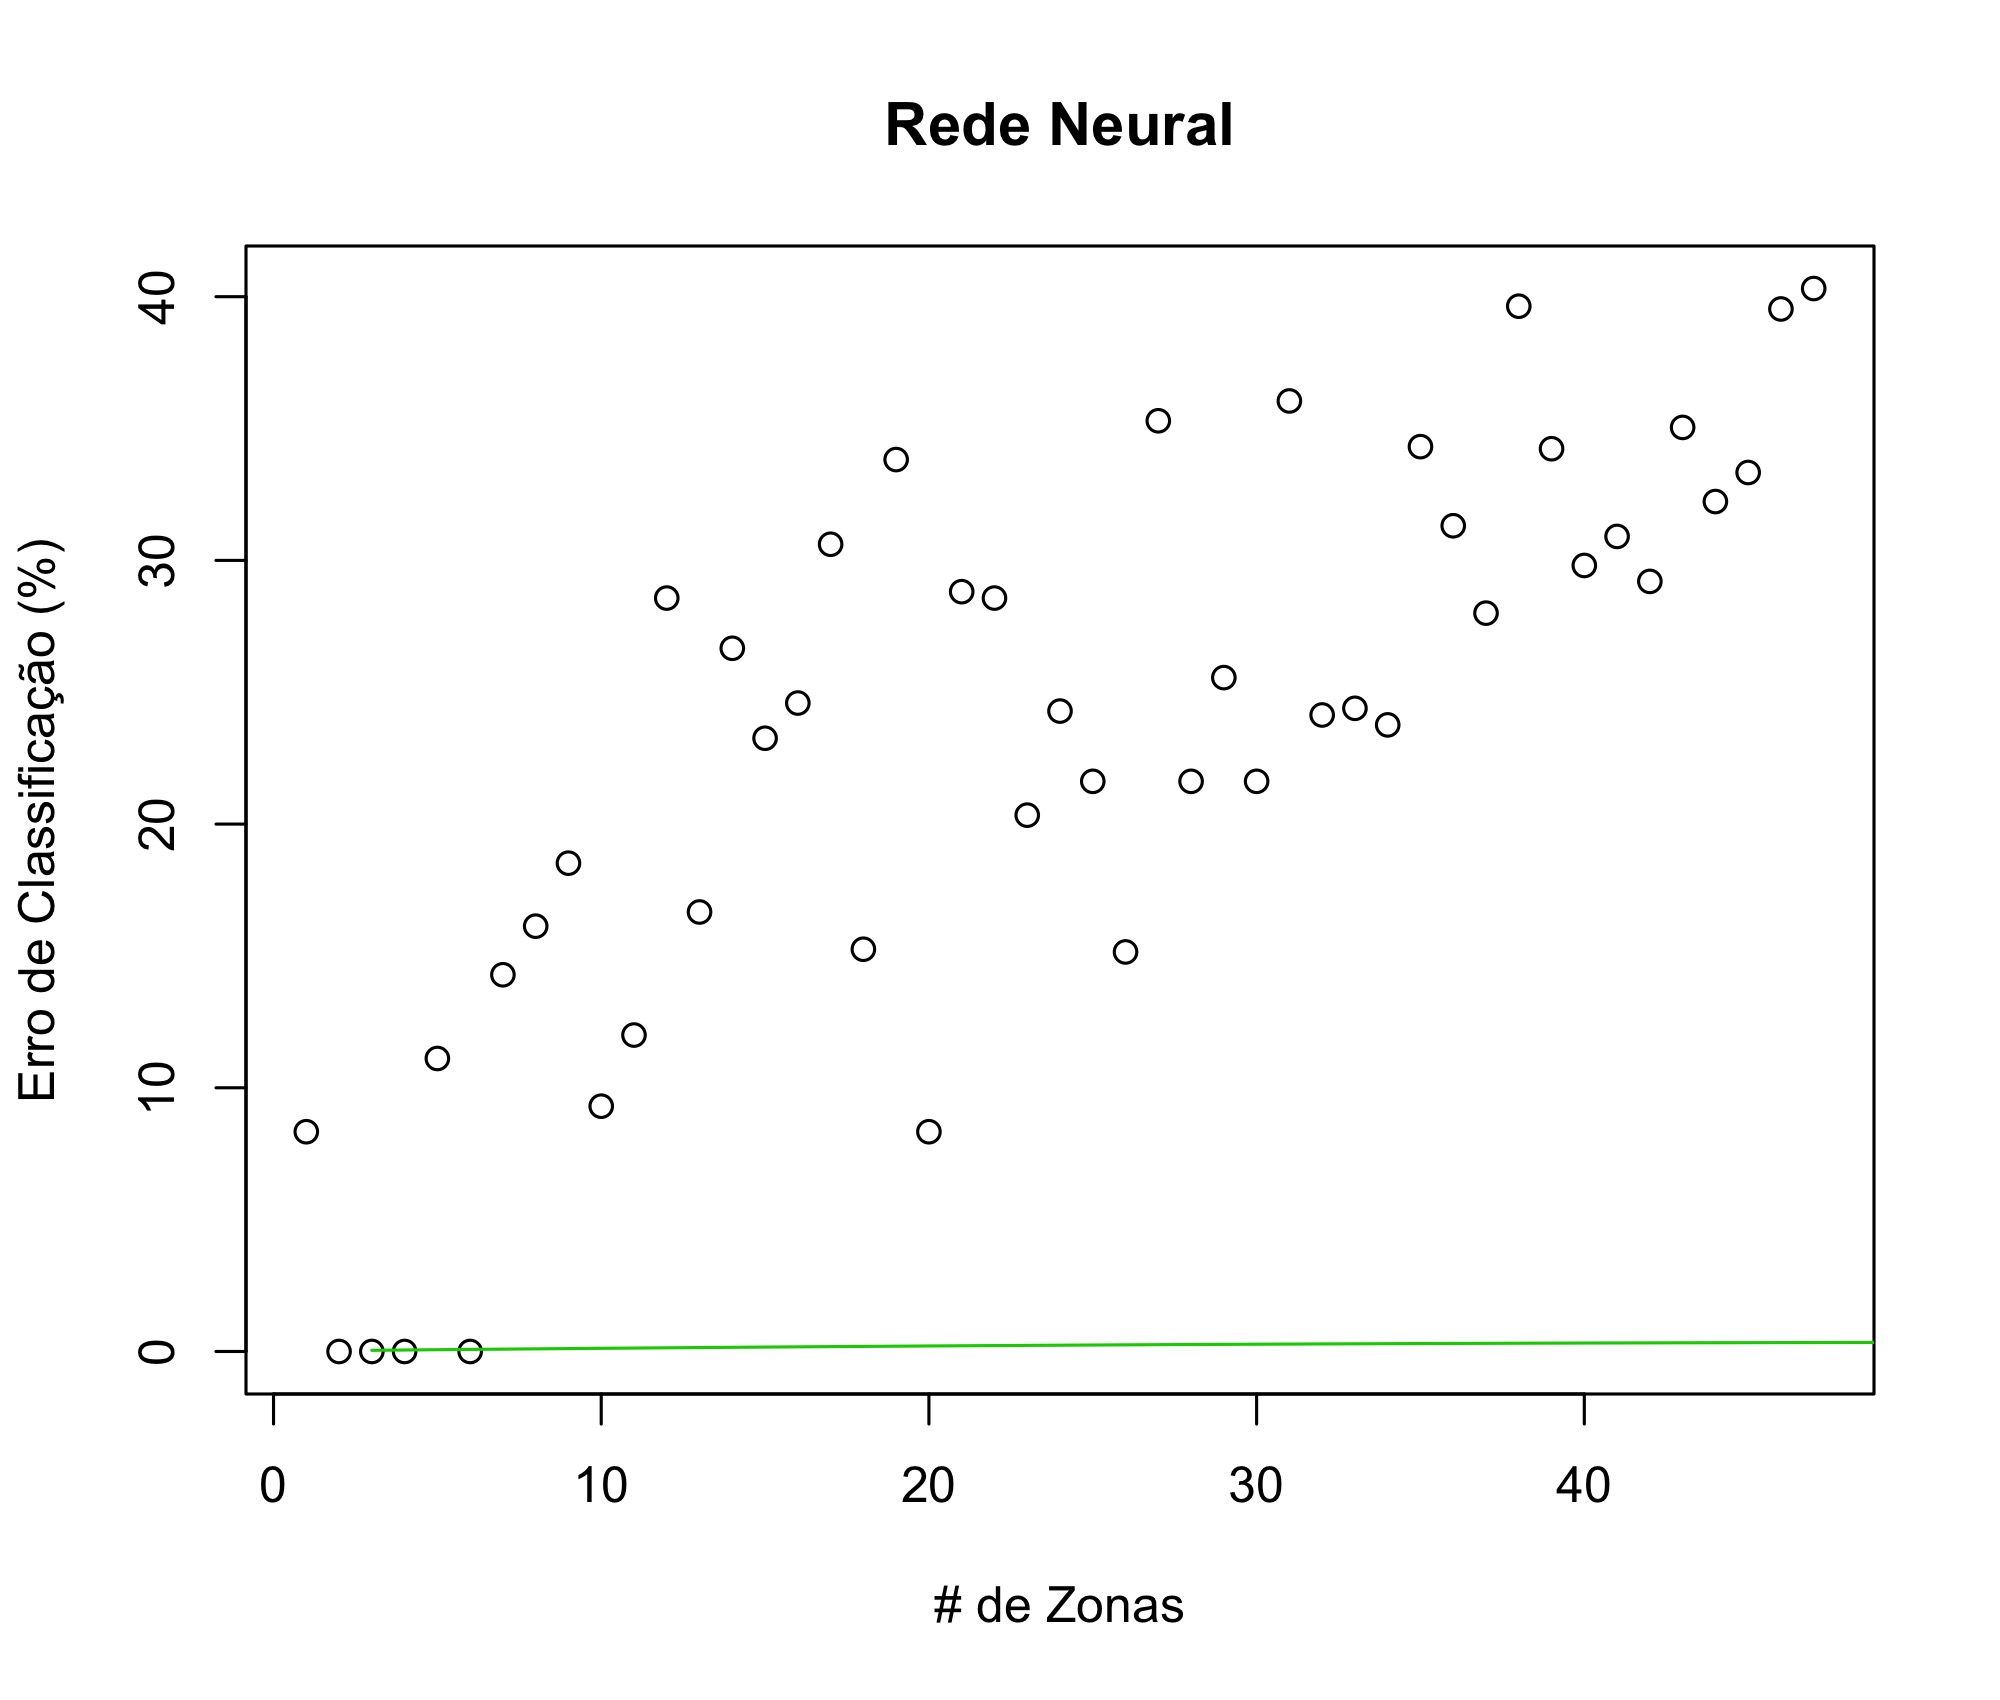
\includegraphics[width=0.9\textwidth]{errorporzonaNN}
\label{fig:zonaNN}

\end{figure}


\begin{figure}[!h]
	\centering
	\caption{Erro do algoritmo KNN para uma quantidade crescente de zonas de classificação.}
  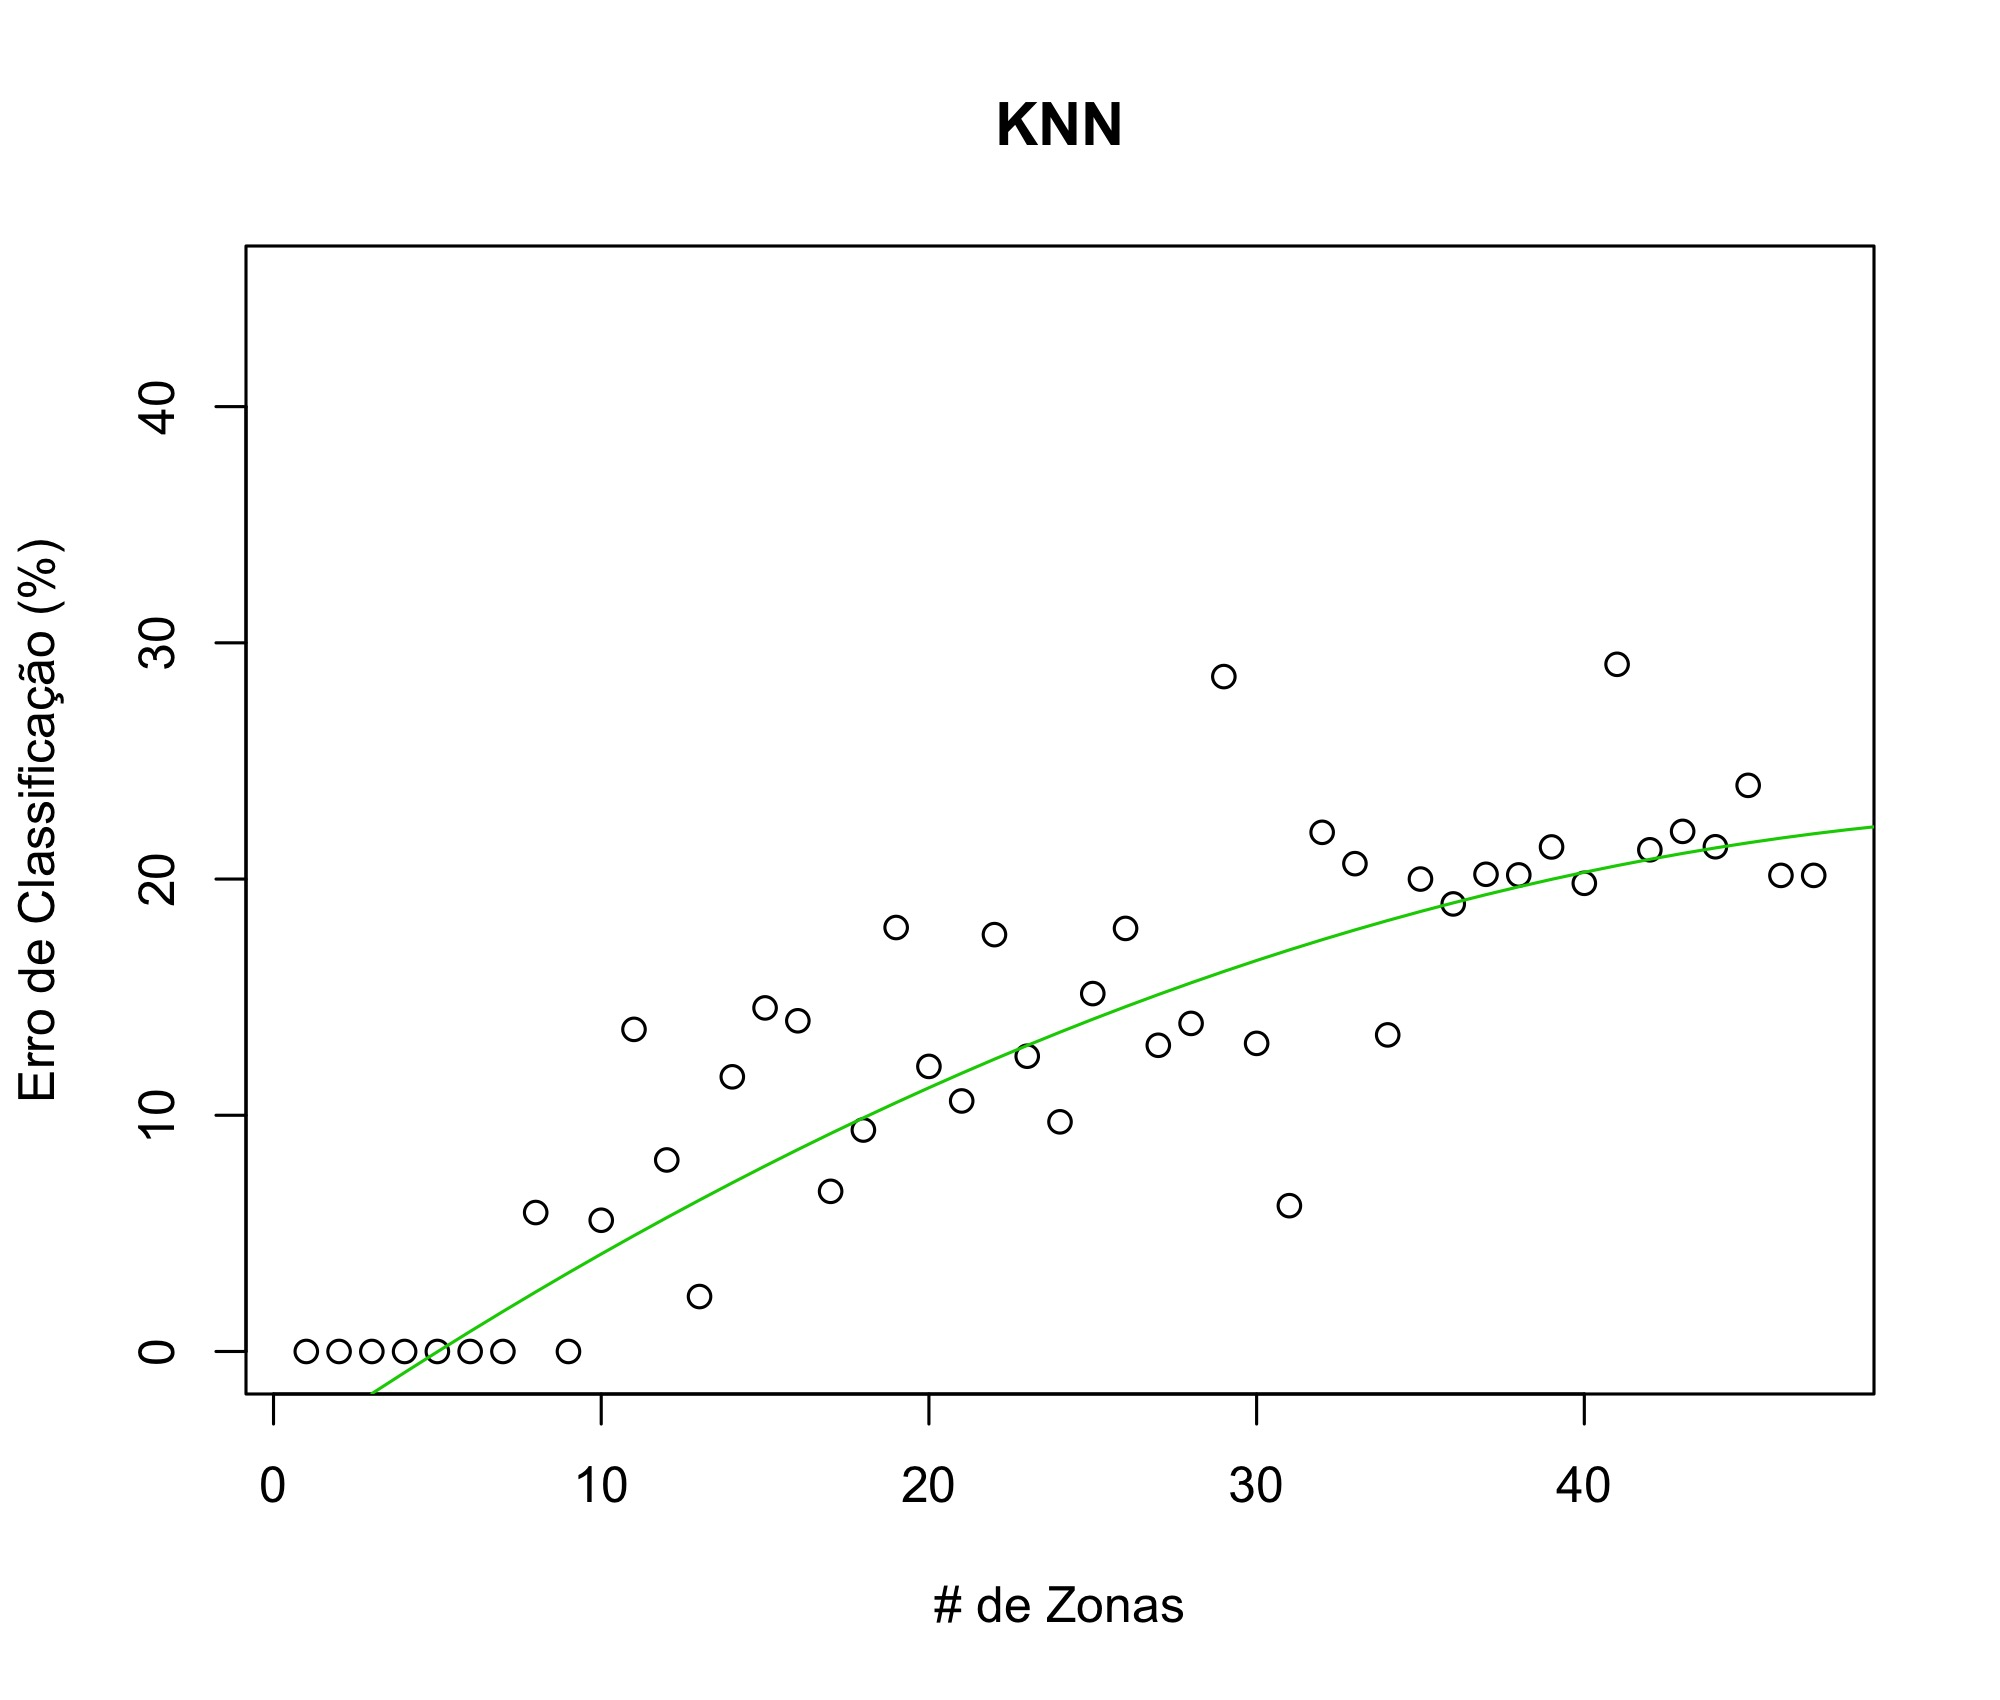
\includegraphics[width=0.9\textwidth]{errorporzonaKNN}
\label{fig:zonaKNN}

\end{figure}



\begin{figure}[!hb]
	\centering
	\caption{Erro do algoritmo de Árvore de Decisão com e sem o Adaboost  para uma quantidade crescente de zonas de classificação.}
  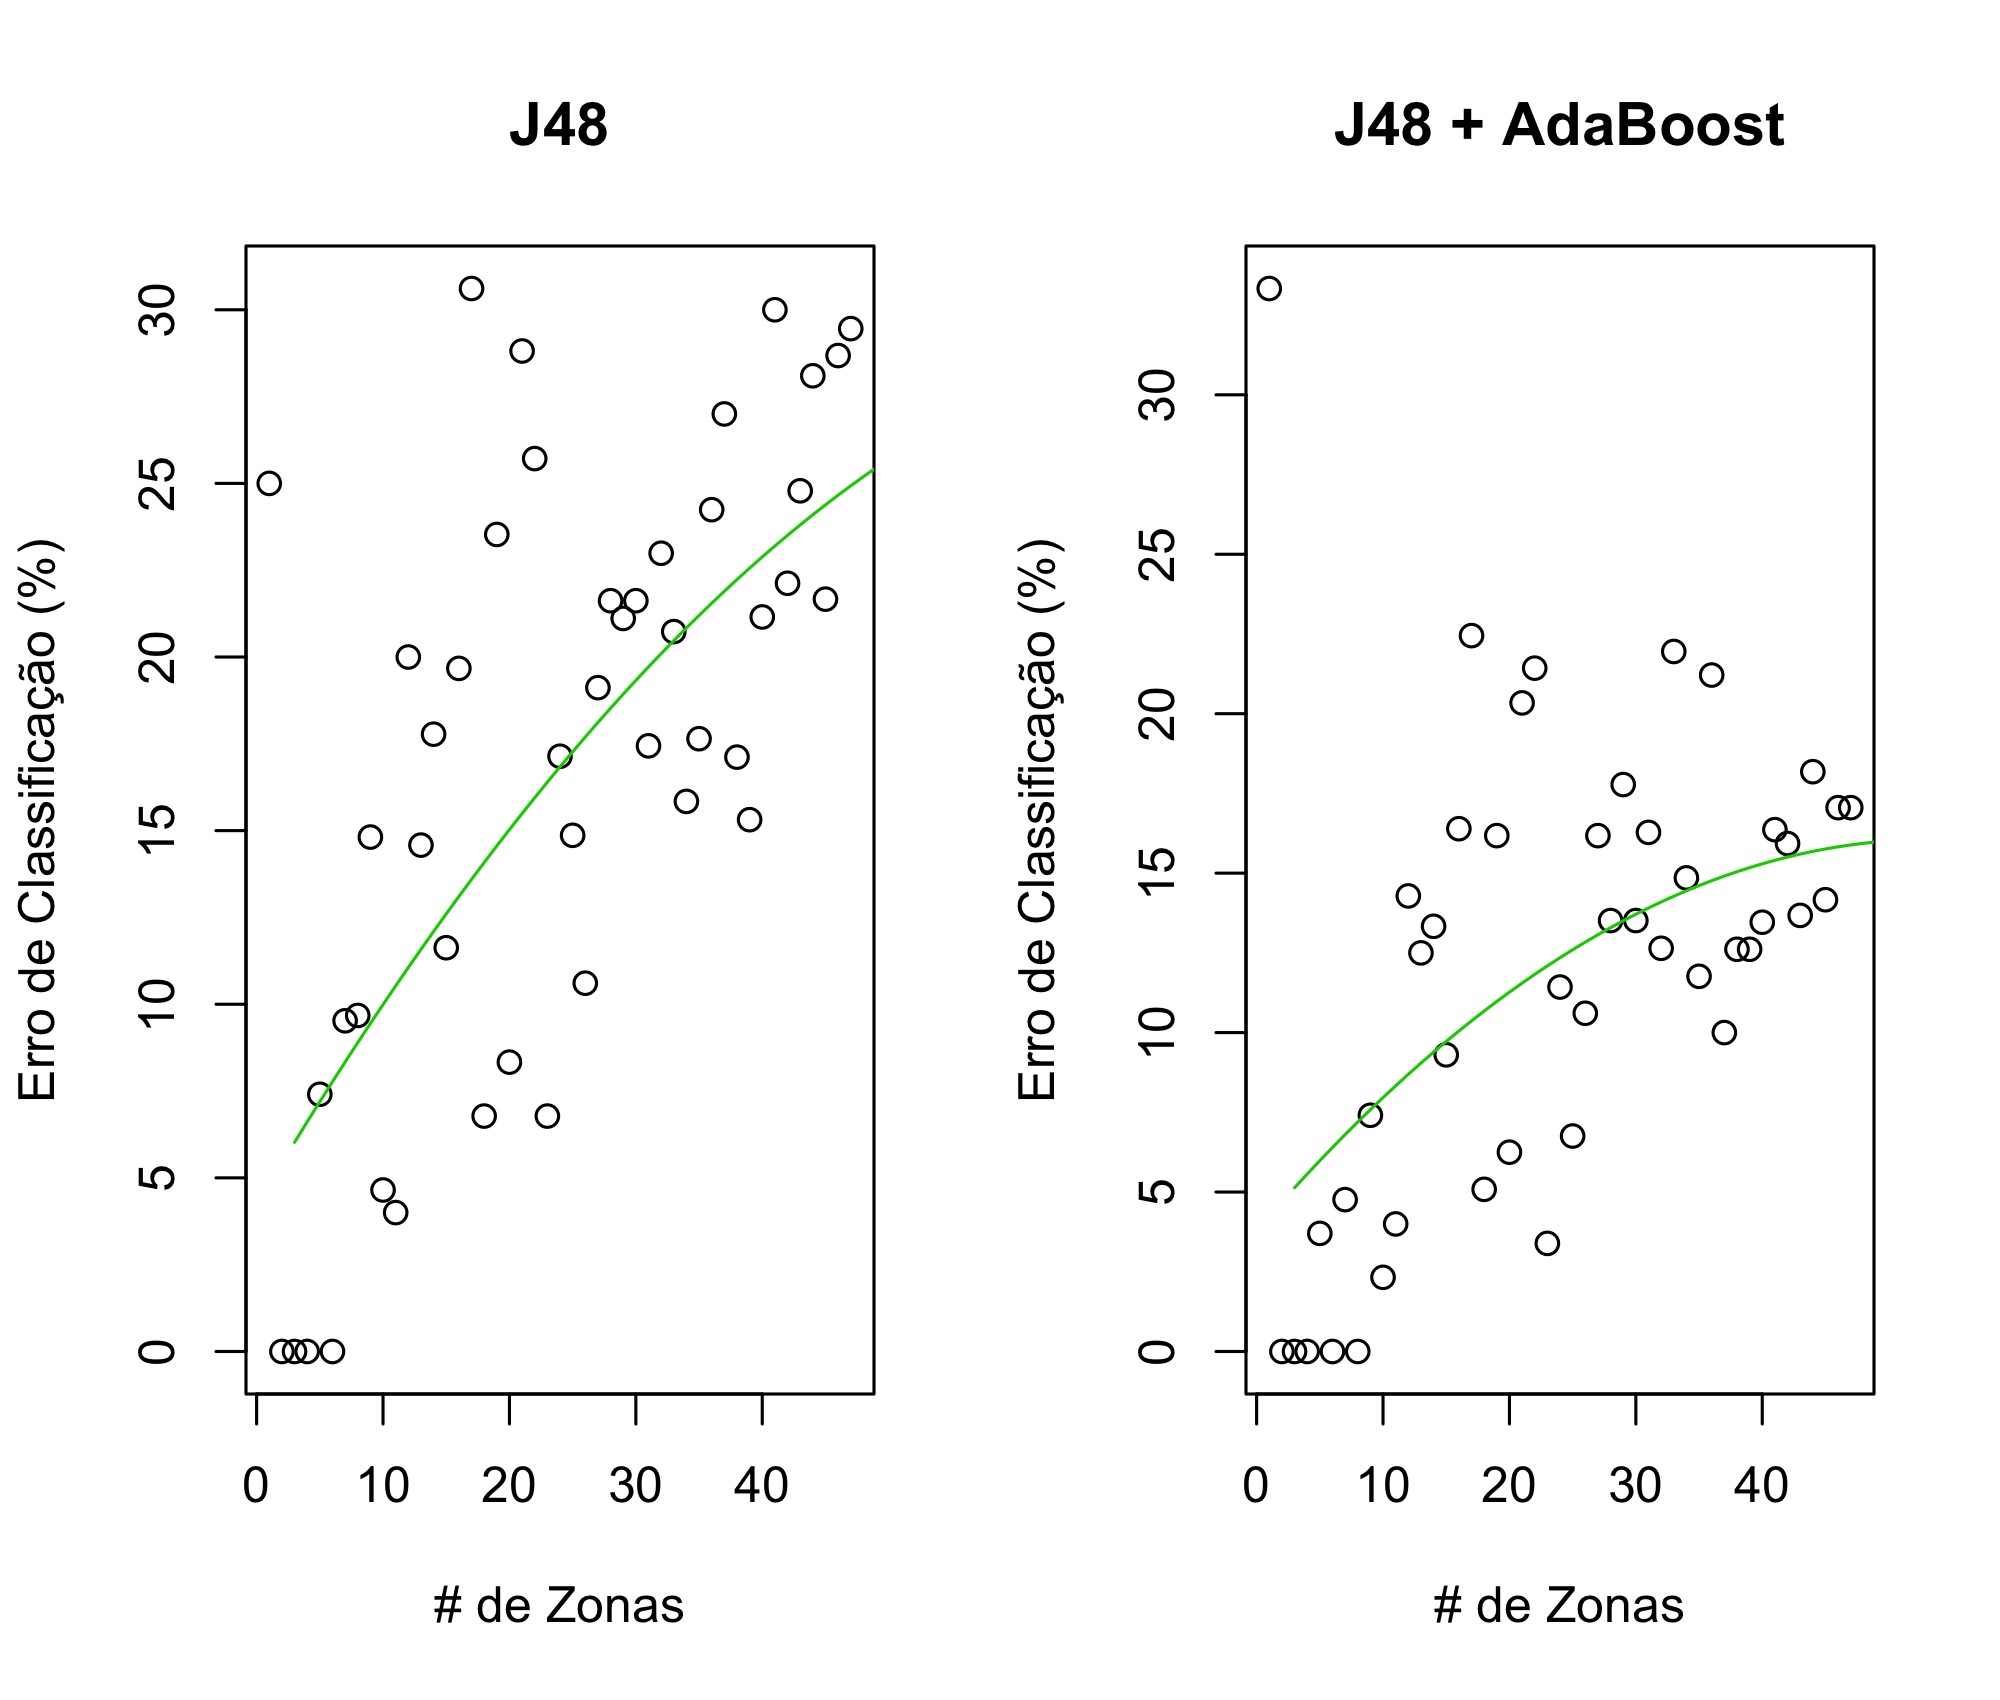
\includegraphics[width=0.9\textwidth]{errorporzonaJ48+Ada}
\label{fig:zonaAda}

\end{figure}

\clearpage


\section{Métodos de Votação}

Os chamados sistemas de \textit{Ensemble Learning} são aqueles em que uma classificação é feita com base em diversos modelos treinados. Em tópicos anteriores foi discutido o uso do algoritmo AdaBoost, que é um método desse tipo para melhorar o poder de classificadores fracos treinando iterativamente diversos modelos fracos progressivamente com os erros do anterior \cite {explainingadaboost}. Porém, para agregar os modelos usados até agora, iremos implementar algo mais simples, porém seguindo a mesma lógica: Sistemas de Votação. Baseados em \cite{Nagi2013}, usaremos diversos métodos para combinar as classificações dos nossos modelos treinados. Em um, usaremos apenas a classe de saída dos modelos, e posteriormente, as probabilidades (\textit{supports}) para cada uma das classes, que também são saídas dos modelos. Esses \textit{supports} podem ser, dependendo do modelo, a probabilidade posterior ou o grau de confiança fornecido pelos algoritmos. Por exemplo, nas redes neurais a saída de um neurônio é a função sigmoide aplicada nas entradas multiplicada pela matriz de pesos da rede, que, por definição, é um número entre 0 e 1 que representa uma probabilidade.




\subsection{Testes com os Métodos de Votação}

Como na sessão de comparação dos modelos, os métodos tem seu erro testado para datasets com um número crescente de zonas aleatórias a serem classificadas. Todos os testes foram feitos com os dados do primeiro andar do prédio 1 do dataset \textit{UJIIndoorLoc} (i.e. BuildingID 1, FloorID 0).




\begin{figure}[!ht]
	\centering
	\caption{Erro do Voto Simples e Voto Ponderado para uma quantidade crescente de zonas de classificação.}
  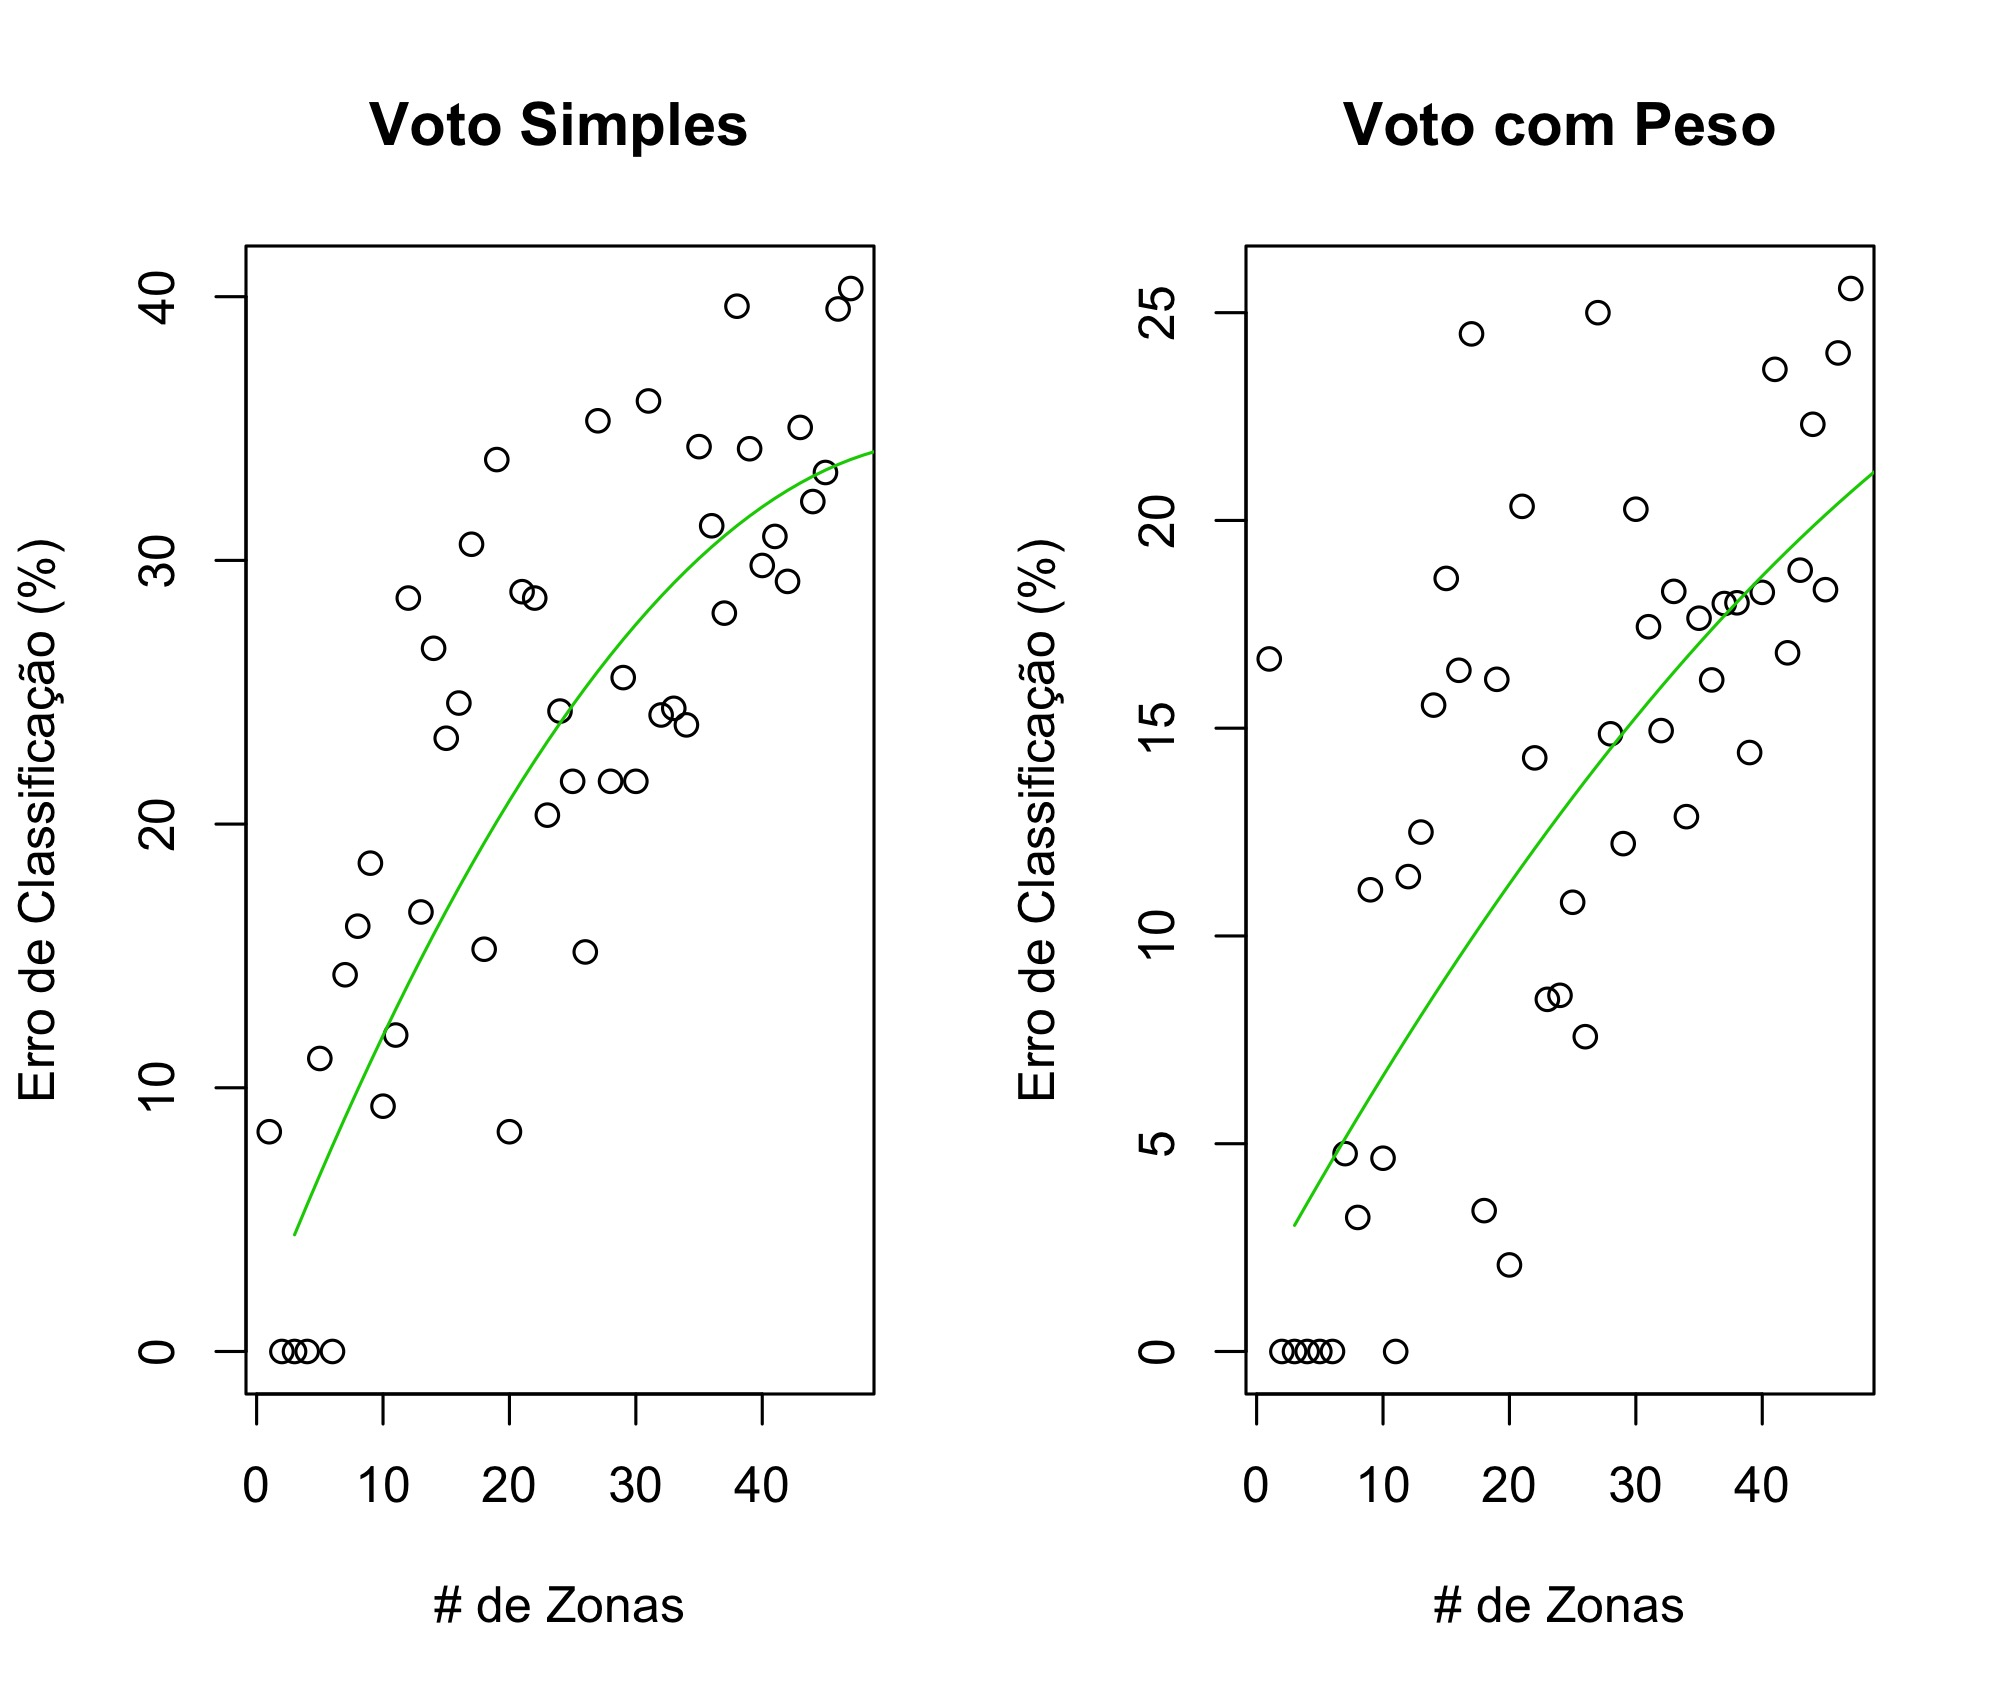
\includegraphics[width=0.9\textwidth]{errorporzonaVotos}
\label{fig:zonaVotos}

\end{figure}



% ========== Referências ==========
% --- IEEE ---
%	http://www.ctan.org/tex-archive/macros/latex/contrib/IEEEtran
%\bibliographystyle{IEEEbib}

% --- ABNT (requer ABNTeX 2) ---
%	http://www.ctan.org/tex-archive/macros/latex/contrib/abntex2
\bibliographystyle{abntex2-alf}

\bibliography{monografia}


% ========== Apêndices (opcional) ==========
\apendice
%\chapter{Alpha}


% ========== Anexos (opcional) ==========
\anexo
%\chapter{}



\end{document}
